\chapter{Unirational surfaces}\label{chap3}

\section{Review on forms of the affine line 
over a field}\label{chap3:chap3-sec1}\pageoriginale\

\subsection{}\label{chap3:1.1}
Throughout this section the ground field $k$ is assumed to be a
nonperfect field of characteristic $p>0$. We denote by $k_{s}$ and
$\overline{k}$ the algebraic separable closure and the algebraic
closure of $k$, respectively. For an integer $n$ we denote by
$k^{p^{n}}$ the sub field $\{\lambda^{p^{n}}|\lambda\in k\}$ of
$\overline{k}$. An irreducible nonsingular affine curve $X$ defined
over $k$ is said to be {\em a $k$-form of the affine line
  $\mathbb{A}^{1}_{k}$} if $\foprod{X}{k'}{k}$ is $k'$-isomorphic to
$\mathbb{A}^{1}_{k}$, for some algebraic extension $k'$ of $k$. It is
a well-known fact that $X$ is $k$-isomorphic to $\mathbb{A}^{1}_{k}$
if $k'$ is taken to be separable over $k$. Thus, we have only to
consider the case where $k'$ is purely inseparable over $k$. We shall
recall several results from \cite{26} and \cite{27} which we need in
the subsequent sections. 

\subsection{}\label{chap3:1.2}
Let $X$ be a $k$-form of $\mathbb{A}^{1}_{k}$ and let $C$ be a
complete normal model of $k(X)$. Then $C$ has only one place
$P_{\infty}$ outside of $X$ which is possibly singular. The $k$-genus
of $C$ is called {\em the genus of}\pageoriginale\ $X$. The function
field $k(X$ is a $k$-form of the rational function field $k(t)$, \iec
$\foprod{k(X)}{k'\cong k'(t)}{k}$  for some algebraic extension $k'$
of $k$. Conversely, given a $k$-form $K$ of the rational function
field $k(t)$, let $C$ be a complete $k$-normal model. Then $K$ is the
function field of a $k$-form of $\mathbb{A}^{1}_{k}$ if and only if
$C$ has at most one singular place. If $C$ has a unique singular place
$P_{\infty}$, $X:=C-P_{\infty}$ is a nontrivial $k$-form of
$\mathbb{A}^{1}_{k}$ (\cf [26; 6.7]). If $C$ is nonsingular $C$ is
$k$-isomorphic to $\mathbb{P}^{1}_{k}$ except possibly when $p=2$ (\cf
[ibid., 6.7.7]); in case $p=2$, if $C$ has a $k$-rational point then
$C$ is $k$-isomorphic to $\mathbb{P}^{1}_{k}$; if $P_{\infty}$ is any
point purely inseparable over $k$ on $C$ then $X:=C-P_{\infty}$ is a
nontrivial $k$-form of $\mathbb{A}^{1}_{k}$.

\subsection{}\label{chap3:1.3}
Let $a$ be an element of $k-k^{p}$ and let $n$ be a positive
integer. Let $\varphi:\mathbb{P}^{1}_{k}\to \mathbb{P}^{n}_{k}$ be the
embedding of $\mathbb{P}^{1}_{k}$ into $\mathbb{P}^{n}_{k}$ given by
$t\mapsto (1,t,\ldots,t^{p^{n}-1},t^{p^{n}}-a)$, where $t$ is an
inhomogeneous parameter of $\mathbb{P}^{1}_{k}$. Let $P_{\infty}$ be
the point of $\mathbb{P}^{1}_{k}$ defined by $t^{p^{n}}=a$. Denote by
$X_{a,n}$ the image $\varphi(\mathbb{P}^{1}_{k}-\{P_{\infty}\})$. Then
we have:

\begin{lemma*}[(\cf {[26; Th.\@ 6.8.1]} ]
\begin{enumerate}
\renewcommand{\theenumi}{\roman{enumi}}
\renewcommand{\labelenumi}{\rm(\theenumi)}
\item Every $k$-rational $k$-form of $\mathbb{A}^{1}_{k}$ is
  $k$-isomorphic to $\mathbb{A}^{1}_{k}$ of $X_{a,n}$ for suitable
  $a\in k-k^{p}$ and $n\in \mathbb{Z}^{+}$.

\item $X_{a,n}$ is a $k$-rational $k$-form of $\mathbb{A}^{1}_{k}$ not
  $k$-isomorphic to $\mathbb{A}^{1}_{k}$.

\item $X_{a,n}$ is $k$-isomorphic to $X_{b,m}$ if and only if $m=n$
  and there exist $\alpha$, $\beta$, $\gamma$, $\delta$ in $k^{p^{n}}$
  such that $\alpha\delta-\beta\gamma\neq 0$ and $(\alpha
  a+\beta)/(\gamma a+\delta)=b$.
\end{enumerate}
\end{lemma*}

\subsection{}\label{chap3:1.4}
\begin{lemma*}[(\cf {[ibid.; 6.8.2 f.]}) ]
  A\pageoriginale\ $k$-form $X$ of $\mathbb{A}^{1}_{k}$ of $k$-genus $1$
  which has a $k$-rational point is $k$-birationally equivalent to an
  affine plane $k$-curve of one of the following types:
  \begin{enumerate}
    \renewcommand{\labelenumi}{\rm(\theenumi)}
  \item $p=3$; $y^{2}=x^{3}+\gamma$ with $\gamma\in k-k^{3}$.
    
  \item $p=2$; $y^{2}=x^{3}+\beta x+\gamma$ with $\beta$, $\gamma\in k$
    such that $\beta\not\in k^{2}$ or $\gamma\not\in k^{2}$.
  \end{enumerate}
  Let $P_{\infty}:=(x=-\gamma^{1/3},y=0)$ in the first case and
  $P_{\infty}:=(x=\beta^{1/2},y=\gamma^{1/2})$ in the second case. Let
  $C$ be a complete $k$-normal model of $k(X)$. Then $X$ is
  $k$-isomorphic to $C-P_{\infty}$.
\end{lemma*}

\subsection{}\label{chap3:4}
A $k$-form $X$ of $\mathbb{A}^{1}_{k}$ is said to be {\em
  hyperelliptic} if the complete $k$-normal model of $k(X)$ is
hyperelliptic.

\subsubsection{}\label{chap3:1.5.1}
\begin{lemma*}[(\cf {[27; Th.\@ 2.2]}) ]
  Let $k$ be a separably closed\footnote{Instead of assuming the
    separable closedness on $k$ it suffices to assume that a $k$-form of
    $\mathbb{A}^{1}_{k}$ has a $k$-rational point.} nonperfect field of
  characteristic $p>2$. Then, a hyperelliptic $k$-form of
  $\mathbb{A}^{1}_{k}$ of $k$-genus $g\geqq 2$ is $k$-birationally
  equivalent to an affine plane curve of the type
  $$
  y^{2}=x^{p^{m}}-a,\quad\text{where}\quad a\in k-k^{p},
  $$
  with $g=(p^{m}-1)/2$. Conversely, the complete $k$-normal model $C$ of
  every such plane curve has a unique singular point $P_{\infty}$, and
  $C-P_{\infty}$ is a $k$-form of $\mathbb{A}^{1}_{k}$ of $k$-genus
  $(p^{m}-1)/2$. 
\end{lemma*}

\subsubsection{}\label{chap3:1.5.2}
\begin{lemma*}[(\cf {[ibid.; Th.\@ 2.3]}) ]
  Let $k$ be a separably closed nonperfect\pageoriginale\ field of
  characteristic $2$. Then a hyperelliptic $k$-form of
  $\mathbb{A}^{1}_{k}$ of $k$-genus $g\geqq 2$ is $k$-birationally
  equivalent to an affine plane curve of one of the following types:
  \begin{enumerate}
    \renewcommand{\theenumi}{\Alph{enumi}}
    \renewcommand{\labelenumi}{\rm(\theenumi)}
  \item $y^{2}+(x^{2^{i}}+a)^{2^{\ell}}y+b=0$, where $i\geqq 0$,
    $\ell\geqq 0$, $a\in k$, $b\in k-\{0\}$; $a\not\in k^{2}$ if $i>0$,
    $b\not\in k^{2}$ if $\ell>0$; and $g=2^{i+\ell}-1$.
    
  \item $y^{2}=x(x+\alpha)^{2g}+E(x)$, where $\alpha\in\overline{k}$,
    $(x+\alpha)^{2g}\in k[x]$, $E(x)\in k[x]$ is an even polynomial of
    degree $2g+2$, and $E(\alpha)\not\in k^{2}$ in case $\alpha\in k$.
  \end{enumerate}
  Conversely, the $k$-normal completion of every curve of type {\em(A)}
  of type {\em(B)}, minus its unique singularity, is a $k$-form of
  $\mathbb{A}^{1}_{k}$; of $k$-genus $=g$ in case {\em(A)}, of $k$-genus
  $\leqq g$ in case {\em(B)}. 
\end{lemma*}

\subsubsection{}\label{chap3:1.5.3}
\begin{lemma*}[(\cf {[ibid.; Th.\@ 2.4]}) ]
  The $k$-forms of $\mathbb{A}^{1}_{k}$ of genus $2$ exist only if the
  characteristic $p$ of the separably closed ground field $k$ is either
  $2$ or $5$. Such a $k$-form is $k$-birationally equivalent to one of
  the following $k$-normal affine plane curves:
  \begin{enumerate}
    \renewcommand{\theenumi}{\Roman{enumi}}
    \renewcommand{\labelenumi}{\rm(\theenumi)}
  \item In case $p=2$:
    $$
    C:y^{2}=x(x+\alpha)^{4}+E(x)
    $$
    where $\alpha^{4}\in k$, $E(x)\in k[x]$ is even of degree $6$, and
    either $\alpha\not\in k$ or $E(\alpha)\not\in k^{2}$.
    
  \item In case $p=5$:
    $$
    D:y^{2}=x^{5}+a,\quad a\in k-k^{5}.
    $$\pageoriginale\
  \end{enumerate}
\end{lemma*}

\subsection{}\label{chap3:1.6}
A $k$ group scheme $G$ is called a $k$-group of Russell type if
$\foprod{G}{k'}{k}$ is $k'$-isomorphic to the additive group scheme
$G_{a,k'}$. The underlying $k$-scheme $\overline{G}$ of a $k$-group
scheme of Russell type is clearly a $k$-form of $\mathbb{A}^{1}_{k}$.

\subsubsection{}\label{chap3:1.6.1}
\begin{lemma*}[(\cf Russell \cite{47}; {[26; 2.7]}) ]
  A $k$-group scheme of Russell type is a $k$-closed subgroup scheme of
  $G^{2}_{a}$ whose underlying scheme is given in $\mathbb{A}^{2}_{k}$
  by an equation
  $$
  y^{p^{n}}=a_{0}x+a_{1}x^{p}+\cdots+a_{r}x^{p^{r}},\quad a_{i}\in~
  k(0\leqq i\leqq r),
  $$
  where $a_{0}\neq 0$ and $a_{i}\not\in k^{p}$ for some $1\leqq i\leqq r$.
\end{lemma*}

\subsubsection{}\label{chap3:1.6.2}
\begin{lemma*}[(\cf Russell \cite{47}; {[26; 6.9.1]}) ]
  Let $X$ be a $k$-form of $\mathbb{A}^{1}_{k}$ and let $C$ be the
  $k$-normal completion of $X$. Assume that $X$ has a $k$-rational point
  $P_{0}$. Then the following conditions are equivalent to each other:
  \begin{enumerate}
    \renewcommand{\theenumi}{\roman{enumi}}
    \renewcommand{\labelenumi}{\rm(\theenumi)}
  \item  $X$ has a $k$-group structure with $P_{0}$ as the neutral
    point.
    
  \item $X$ is isomorphic to the underlying scheme of a $k$-group of
    Russell type.
    
  \item $\Aut_{k_{s}}(\foprod{C}{k_{s}}{k})$ is an infinite group.
  \end{enumerate}
\end{lemma*}

\subsubsection{}\label{chap3:1.6.3}
\begin{remark*}
  With the notations of \ref{chap3:1.6.2},
  $\Aut_{k_{s}}(\foprod{C}{k_{s}}{k})=\Aut_{k_{s}}(\foprod{X}{k_{s}}{k})$
  if $X$ is not $k$-rational (\cf [27; 3.1.1]). The function field
  $k(G)$ of a $k$-group $G$ of Russell type is rational if\pageoriginale\
  and only if $p=2$ and $G$ is $k$-isomorphic to an affine plane curve
  $$
  y^{2}=x+ax^{2}\quad\text{with}\quad a\in k-k^{2}.
  $$
  If $p>2$, the underlying $k$-scheme of a $k$-group of Russell type is
  not hyperelliptic (\cf [27; Cor.\@ 3.3.2]).
\end{remark*}

\section{Unirational quasi-elliptic surfaces}\label{chap3:chap3-sec2}\pageoriginale\

\subsection{}\label{chap3:2.1}

Throughout this section, the ground field $k$ is assumed to be an
algebraically closed field of characteristic $p>0$. A nonsingular
projective surface $X$ defined over $k$ is called {\em a
  quasi-elliptic surface} if there exists a morphism $f:X\to C$ from
$X$ to a nonsingular projective curve $C$ such that almost all fibers
of $f$ are irreducible singular rational curves of arithmetic genus
$1$ (\cf \cite{9}, \cite{39}). According to Tate \cite{55}, such
surfaces can occur only in the case where the characteristic $p$ is
either $2$ or $3$, and almost all fibers of $f$ have single ordinary
cusps. Thus, the generic fiber $X_{\mathscr{R}}$ of $f$, minus the
unique singular point, is a $\mathscr{R}$-form of $\mathbb{A}^{1}$ of
$\mathscr{R}$-genus $1$, where $\mathscr{R}$ is the function field of
$C$ over $k$. On the other hand, $X$ is unirational over $k$ if and
only if $C$ is a rational curve. {\em We assume in this section that
  every quasi-elliptic surface has a rational cross-section}, \iec
there is a rational mapping $s:C\to X$ such that $f\cdot
s=\id_{C}$. Our ultimate purpose is to prove the following two
theorems.

\subsubsection{}\label{chap3:2.1.1}
\begin{theorem*}
  Let $k$ be an algebraically closed field of characteristic $3$. Then
  any unirational quasi-elliptic surface with a rational cross-section
  defined over $k$ is birational to a hyper-surface in
  $\mathbb{A}^{3}_{k}:t^{2}=x^{3}+\varphi(y)$ with $\varphi(y)\in k[y]$
  of degree prime to $3$. Let $K:=k(t,x,y)$ be the algebraic function
  field of an affine hypersurface of the above type, let
  $m=[\frac{d}{6}]$ and let $\widehat{H}$ be the (nonsingular) minimal
  model of $K$ when $K$ is not rational over $k$\footnote{Note that if
    $K$ is ruled and unirational then $K$ is rational. Hence if $K$ is
    not rational $K$ has the minimal model.}. Moreover,\pageoriginale\ if
  $d\geqq 7$ assume that the following conditions hold:
  \begin{enumerate}
    \renewcommand{\labelenumi}{\rm(\theenumi)}
  \item For every root $\alpha$ of $\varphi'(y)=\dfrac{d\varphi}{dy}=0$,
    $v_{\alpha}(\varphi(y)-\varphi(\alpha))\leqq 5$, where $v_{\alpha}$
    is the $(y-\alpha)$-adic valuation of $k[y]$ with
    $v_{\alpha}(y-\alpha)=1$.
    
  \item If, moreover,
    $\varphi(y)-\varphi(\alpha)=a(y-\alpha)^{3}+${\em (terms of higher
    degree in $y-\alpha$)} for some root $\alpha$ of $\varphi'(y)=0$ and
    $a\in k^{\ast}$ then
    $v_{\alpha}(\varphi(y)-\varphi(\alpha)-a(y-\alpha)^{3})\leqq 5$.
  \end{enumerate}
  Then we have the following:
  \begin{enumerate}
    \renewcommand{\theenumi}{\roman{enumi}}
    \renewcommand{\labelenumi}{\rm(\theenumi)}
  \item If $m=0$, \iec $d\leqq 5$, then $K$ is rational over $k$. If
    $d\geqq 7$, $K$ is not rational over $k$, and the minimal model
    $\widehat{H}$ exists.
    
  \item If $m=1$, \iec $7\leqq d\leqq 11$, then $\widehat{H}$ is a
    $K3$-surface.
    
  \item If $m>1$, \iec $d\geqq 13$, then
    $p_{a}(\widehat{H})=p_{g}(\widehat{H})=m$, $\dim
    H^{1}(\widehat{H},\mathscr{O}_{\widehat{H}})=0$, the $r$-genus
    $P_{r}(\widehat{H})=r(m-1)+1$ for every positive integer $r$ and the
    canonical dimension $\kappa(H)=1$.
  \end{enumerate}
\end{theorem*}

\subsubsection{}\label{chap3:2.1.2}
\begin{theorem*}
  Let $k$ be an algebraically closed field of characteristic $2$. Then
  any unirational quasi-elliptic surface with a rational cross-section
  defined over $k$ is birational to a hyper-surface in
  $\mathbb{A}^{3}_{k}:t^{2}=x^{3}+\psi(y)x+\phi(y)$ with $\phi(y)$,
  $\psi(y)\in k[y]$. Conversely, let $K:=k(t,x,y)$ be an algebraic
  function field of dimension $2$ generated by $t$, $x$, $y$ over $k$
  such that $t^{2}=x^{3}+\phi(y)$ with $\phi(y)=y\varphi(y)^{2}\in
  k[y]$\footnote{With no loss of generality, we may write $\phi(y)$ in
    the form $\phi(y)=y\varphi(y)^{2}$.} and $d=\deg_{y}\varphi$. Let
  $m=[\dfrac{d}{3}]$. Assume moreover that, for every $\alpha\in k$, if
  we write $\phi(y+\alpha)={\displaystyle{\mathop{\sum}_{i\geqq
        0}}}a_{i}y^{i}$ then one of $a_{1}$, $a_{3}$ and $a_{5}$ is
  nonzero. Then we have the following:
  \begin{enumerate}
    \renewcommand{\theenumi}{\roman{enumi}}
    \renewcommand{\labelenumi}{\rm(\theenumi)}
  \item If $m=0$, \iec $0\leq d\leqq 2$, $K$ is rational over $k$. If
    $m>0$,\pageoriginale\ $K$ is not rational over $k$, and the minimal
    model $\widehat{H}$ of $K$ over $k$ exists.
    
  \item If $m=1$, \iec $3\leqq d\leqq 5$, then $\widehat{H}$ is a
    $K3$-surface.
    
  \item If $m>1$, \iec $d\geqq 6$, then
    $p_{a}(\widehat{H})=p_{q}(\widehat{H})=m$, $\dim
    H^{1}(\widehat{H},\mathscr{O}_{\widehat{H}})=0$, the $r$-genus
    $P_{r}(\widehat{H})=r(m-1)+1$ for every positive integer $r$ and the
    canonical dimension $\kappa(\widehat{H})=1$.
  \end{enumerate}
\end{theorem*}

Proofs of both theorems will be given after some preparations on
double coverings.

\subsection{}\label{chap3:2.2}
Let $X$, with $f:X\to C$, be a quasi-elliptic surface defined over $k$
and let $\mathscr{R}$ be the function field of $C$ over $k$. Then the
generic fiber $X_{\mathscr{R}}$ of $f$ is an irreducible normal
projective curve over $\mathscr{R}$ with arithmetic genus
$p_{a}(X_{\mathscr{R}})=1$ and geometric genus $0$. Hence
$X_{\mathscr{R}}$ has only one singular point, whose multiplicity is
$2$. Let $\mathscr{R}_{s}$ be a separable algebraic closure of
$\mathscr{R}$. By Chevalley [12; Th.\@ 5, p.99],
$\foprod{X}{\mathscr{R}_{s}}{\mathscr{R}}$ is then a normal projective
curve of arithmetic genus $1$. This implies that the characteristic
$p$ of $k$ must be either $2$ or $3$ by virtue of Tate \cite{55}, and
that the singular point of $X_{\mathscr{R}}$ is a one-place point of
multiplicity $2$, which is rational over a purely inseparable
extension of $\mathscr{R}$. Therefore, general fibers of $f$ have
single ordinary cusps.

Let $\Gamma$ be the closure in $X$ of the unique singular point of
$X_{\mathscr{R}}$. Let $f_{\Gamma}:\Gamma\to C$ be the restriction of
$f$ onto $\Gamma$. Since the singular point of $X_{\mathscr{R}}$ is a
one-plance point, $f_{\Gamma}$ is a generically one-to-one
morphism. Hence $\deg f_{\Gamma}$ is a power $p^{n}$ of the
characteristic $p$, and, for a fiber $f^{-1}(p)$ of $f$ such that
$f^{-1}(P)$ meets\pageoriginale\ $\Gamma$ at a simple point of
$\Gamma$, the intersection number $(\Gamma\cdot f^{-1}(P))$ must be
$2$ or $3$ because $\Gamma\cap f^{-1}(P)$ is an ordinary cusp. Hence,
$n=1$ and $(\Gamma\cdot f^{-1}(P))=p$. On the other hand, $\Gamma$ is
a nonsingular curve. Indeed, if $\Gamma$ has a singular point $Q$,
then $(\Gamma\cdot f^{-1}(f(Q)))\geqq 4$, which contradicts the fact
that $(\Gamma\cdot f^{-1}(f(Q)))=p\leqq 3$.

Assume that $f$ has a rational cross-section $D$; by virtue of [17, IV
  (2.8.5)] $D$ is in fact extended to a regular cross-section of
$f$. This is equivalent to saying that the generic fiber
$X_{\mathscr{R}}$ of $f$ has a $\mathscr{R}$-rational point. With the
unique singular point deleted off, $X_{\mathscr{R}}$ becomes a
$\mathscr{R}$-form of the affine line $\mathbb{A}^{1}$ of
$\mathscr{R}$-genus $1$ with a $\mathscr{R}$-rational point. Such a
form is birationally equivalent to one of the following affine plane
curves (\cf \ref{chap3:1.4}):
\begin{enumerate}
\renewcommand{\theenumi}{\roman{enumi}}
\renewcommand{\labelenumi}{(\theenumi)}
\item If $p=3$, $t^{2}=x^{3}+\gamma$ with
  $\gamma\in\mathscr{R}-\mathscr{R}^{3}$. 

\item If $p=2$, $t^{2}=x^{3}+\beta x+\gamma$ with $\beta$, $\gamma\in
  \mathscr{R}$ such that $\beta\not\in \mathscr{R}^{2}$ or
  $\gamma\not\in \mathscr{R}^{2}$.
\end{enumerate}
The surface $X$ is unirational over $k$ if and only if $C$ is
rational. Indeed, the ``only if'' part is apparent by L\"uroth's
theorem; the ``if'' part is also easy to see: If $p=3$,
$\foprod{\mathscr{R}^{1/3}}{k(X)}{\mathscr{R}}$ is rational over $k$,
and if $p=2$, $\foprod{\mathscr{R}^{1/2}}{k(X)}{\mathscr{R}}$ is
rational over $k$. Thus, if $f:X\to C$ is a unirational quasi-elliptic
surface defined over $k$ with a rational cross-section, the function
field $\mathscr{R}$ of $C$ over $k$ is a rational function field
$k(y)$ over $k$, and $X$ is $k$-birationally equivalent to one of the
following hypersurfaces in the affine $3$-space $\mathbb{A}^{3}_{k}$:
\begin{enumerate}
\renewcommand{\theenumi}{\roman{enumi}}
\renewcommand{\labelenumi}{(\theenumi)$'$}
\item If $p=3$, $t^{2}=x^{3}+\varphi(y)$ with $\varphi(y)\in k[y]$,
  where $d:=\deg_{y}\varphi$\pageoriginale\ is prime to $3$.

\item If $p=2$, $t^{2}=x^{3}+\psi(y)x+\phi(y)$ with $\phi(y)$,
  $\psi(y)\in k[y]$.
\end{enumerate}


\subsection{}\label{chap3:2.3}
We shall recall and apply the canonical divisor formula for elliptic
or quasi-elliptic fibrations (\cf \cite{10}). Let $f:X\to C$ be a
morphism form a nonsingular projective surface $X$ to a nonsingular
projective curve $C$ such that almost all fibers of $f$ are
irreducible curves of arithmetic genus $1$. A fiber $f^{-1}(P)$ of $f$
is called {\em a reducible fiber} of $f$ if $f^{-1}(P)$ has either not
less than two (distinct) irreducible components or a single
irreducible component with multiplicity $\geqq 2$; a fiber $f^{-1}(P)$
is called {\em a multiple fiber} if, when we write $f^{-1}(P)$ in the
form $f^{-1}(P)={\displaystyle{\mathop{\sum}_{i}}}n_{i}C_{i}$ with
irreducible components $C_{i}$ and positive integers $n_{i}$, the
greatest common divisor $q$ of $n_{i}$'s is greater than $1$. Then,
writing $m_{i}=n_{i}/q$,
${\displaystyle{\mathop{\sum}_{i}}}m_{i}C_{i}$ is called {\em the
  reduced form} of a multiple fiber $f^{-1}(P)$. On the other hand, an
elliptic or quasi-elliptic fibration $f:X\to C$ is said to be {\em
  relatively minimal} if each fiber of $f$ contains no exceptional
components. Given an elliptic or quasi-elliptic fibration $f:X\to C$
we can always find a fibration $f_{0}:X_{0}\to C$ such that
$f_{0}\cdot\sigma=f$, where $\sigma:X\to X_{0}$ is the contraction of
exceptional components contained in the fibers. With these definitions
set down, we have the following:

\subsubsection{}\label{chap3:2.3.1}
\begin{lemma*}[(\cf \cite{9}, \cite{10}) ]
  Let $f:X\to C$ be a relatively minimal elliptic or quasi-elliptic
  surface. Let $\{m_{i}Z_{i};i\in I\}$ be the set of all multiple fibers
  of $f$, where $Z_{i}$ is the reduced form. Then we have: 
  $$
  \omega_{X}\cong f^{\ast}(S)\otimes
  \mathscr{O}_{X}(\sum_{i}a_{i}Z_{i})\quad\text{and}\quad S\cong
  \mathscr{O}_{C}\otimes L^{-1},
  $$\pageoriginale\
  where: {\rm(i)} $0\leqq a_{i}\leqq m_{i}-1$, {\rm(ii)} $L$ is an
  invertible sheaf on $C$ defined by either $f_{\ast}\omega_{X}\cong
  \omega_{C}\otimes L^{-1}$ or $R^{1}f_{\ast}\mathscr{O}_{X}\cong
  L\oplus T$, $T$ being a torsion sheaf on $C$. Let $t$ be the length of
  $T$. Then we have 
  $$
  \deg (S)=\chi(\mathscr{O}_{X})-2\chi(\mathscr{O}_{C})+t.
  $$
  For a point $P$ on $C$, $T_{P}\neq 0$ if and only if
  $H^{0}(f^{-1}(P),\mathscr{O}_{X})\varsupsetneqq k$, which implies that
  $f^{-1}(P)$ is an exceptional multiple fiber\footnote{a wild fiber, in
    other words (\cf \cite{10}).}. 
\end{lemma*}

\subsubsection{}\label{chap3:2.3.2}
A key result in proving the stated theorems is the following
\begin{lemma*}
Let $f:X\to C$ be a unirational quasi-elliptic surface with a regular
cross-section $D$. Assume that $X$ is relatively minimal. Then the
following results hold:
\begin{enumerate}
\renewcommand{\labelenumi}{\rm(\theenumi)}
\item $f$ has no multiple fibers.

\item $\chi(\mathscr{O}_{X})=-(D^{2})$.

\item If $\chi(\mathscr{O}_{X})\leqq 1$, $X$ is rational over $k$; if
  $\chi(\mathscr{O}_{X})=2$ then $X$ is a $K3$-surface; if
  $\chi(\mathscr{O}_{X})\geqq 3$ then $p_{a}(X)=p_{q}(X)$, $\dim
  H^{1}(X,\mathscr{O}_{X})=0$, the $r$-genus
  $P_{r}(X)=r(\chi(\mathscr{O}_{X})-2)+1$, and the canonical dimension
  $\kappa(X)=1$. 
\end{enumerate}
\end{lemma*}

\begin{proof}
\begin{enumerate}
\renewcommand{\labelenumi}{(\theenumi)}
\item is obvious because $f$ has a cross-section. 

\item Since there are no multiple fibers in the fibration $f$,
  $a_{i}=0$ for every $i$ and $t=0$ in the canonical divisor formula
  in \ref{chap3:2.3.1}. Since $C$ is a rational curve we know that
  $\omega_{X}\cong
  f^{\ast}\mathscr{O}_{C}(\chi(\mathscr{O}_{X})-2)$. Since $D$ is a
  cross-section of $f$, the arithmetic genus formula on
  $X$\pageoriginale\ applied to a nonsingular rational curve $D$ tells
  us:
$$
-2=(D^{2})+(D\cdot K_{X})=(D^{2})+\chi(\mathscr{O}_{X})-2.
$$
Hence, $\chi(\mathscr{O}_{X})=-(D^{2})$ 

\item For a positive integer $r$, the $r$-genus $P_{r}(X)$ is given by
$$
P_{r}(X)=\dim H^{0}(X,\omega^{\otimes r}_{X})=\dim
H^{0}(C,\mathscr{O}_{C}(r(\chi(\mathscr{O}_{X})-2))). 
$$
If $\chi(\mathscr{O}_{X})\leqq 1$, $P_{r}(X)=0$ for every $r>0$,
whence $P_{12}(X)=0$. This implies that $X$ is ruled (\cf
\cite{10}). Since $X$ is unirational, $X$ is rational. If
$\chi(\mathscr{O}_{X})=2$, we have $\omega_{X}\cong
\mathscr{O}_{X}$. Then $X$ is a $K3$-surface (\cf \cite{9},
\cite{10}). If $\chi(\mathscr{O}_{X})\geqq 3$,
$P_{r}(X)=r(\chi(\mathscr{O}_{X})-2)+1$. Hence the canonical dimension
$\kappa(X)$ is equal to $1$, and
$p_{g}(X)=\chi(\mathscr{O}_{X})-1=p_{a}(X)$. Therefore, $\dim
H^{1}(X,\mathscr{O}_{X})=0$.
\end{enumerate}
\end{proof}

\subsubsection{}\label{chap3:2.3.3}
\begin{coro*}
  Let $f:X\to C$ be a relatively minimal, unirational, quasi-elliptic
  surface defined over $k$ with a regular cross-section. If $X$ is not
  rational over $k$ then $X$ is a minimal (nonsingular) model.
\end{coro*}

\begin{proof}
Set $e:=\chi(\mathscr{O}_{X})-2$. Then $K_{X}\sim ef^{-1}(P)$ for a
point on $C\cong \mathbb{P}^{1}_{k}$. If $X$ is not rational over $k$
we know by \ref{chap3:2.3.2} that $e\geqq 0$. Then the canonical linear
system $|K_{X}|$ has no fixed components, which implies that $X$
contains no exceptional curve of the first kind. $X$ is therefore a
minimal nonsingular model.
\end{proof}

\subsubsection{}\label{chap3:2.3.4}
\begin{lemma*}
  Let $f:X\to C$ be a relatively minimal quasi-elliptic surface with a
  rational cross-section, and let
  $D={\displaystyle{\mathop{\sum}_{i}}}n_{i}E_{i}$ be\pageoriginale\ a
  reducible fiber (having not less than two components). Then every
  component $E_{i}$ is a nonsingular projective rational curve with
  $(E^{2}_{i})=-2$. 
\end{lemma*}

\begin{proof}
For every $i$, $(E_{i}\cdot
D)=n_{i}(E^{2}_{i})+{\displaystyle{\mathop{\sum}_{j\neq
      i}}}n_{j}(E_{i}\cdot E_{j})=0$. Since $D$ is connected,
$(E^{2}_{i})<0$ for every $i$. Since $K_{X}\sim f^{\ast}(S)$ for some
divisor $S$ on $C$ as we have seen in \ref{chap3:2.3.1}, $(E_{i}\cdot
K_{X})=0$. Then $p_{a}(E_{i})=\dfrac{1}{2}(E^{2}_{i})+1\geqq 0$,
whence $(E^{2}_{i})=-2$ and $p_{a}(F_{i})=0$.
\end{proof}


\subsection{}\label{chap3:2.4}
Throughout the paragraphs \ref{chap3:2.4} $\sim$ \ref{chap3:2.7}, we shall assume
that $k$ is an algebraically closed field of characteristic $p\geqq
0$. Let $\varphi(y)$ be a polynomial in $y$ of degree $d\geqq 3$ with
coefficients in $k$ such that $A(x,y):=x^{3}+\varphi(y)$ is an
irreducible polynomial. We assume that $\varphi(y)$ contains no
monomial terms of degree congruent to zero modulo $3$ if $p=3$, and
that $\varphi(y)$ contains no monomial terms of degree congruent to
zero modulo $2$ if $p=2$. Consider a hyper surface $t^{2}=A(x,y)$ in
the projective $3$-space $\mathbb{P}^{3}_{k}$, which is birational to
a double covering of $F_{0}:=\mathbb{P}^{1}_{k}\times
\mathbb{P}^{1}_{k}$. Let $K:=k(t,x,y)$. Let $H_{0}$ be the
normalization of $F_{0}$ in $K$, and let $\rho_{0}:H_{0}\to F_{0}$ be
the normalization morphism. With the above notations and assumptions
we shall show the following:

\subsubsection{}\label{chap3:2.4.1}
\begin{lemma*}
  Let $Q$ be a point on $H_{0}$, and let $P:=\rho_{0}(Q)$. If $P$ is not
  a singular point of $C$ then $Q$ is a simple point of $H_{0}$, where
  $C$ is a closed irreducible curve on $F_{0}$ defined by the equation
  $A(x,y)=0$. 
\end{lemma*}

\subsubsection{}\label{chap3:2.4.2}
In order to prove the above lemma we need 

\begin{lemma*}
Let\pageoriginale\ $A(x,y)$ be a nonzero irreducible polynomial in
$k[x,y]$ such that $A(0,0)=0$, and let $U$ be a hyper surface in the
affine $(t,x,y)$-space $\mathbb{A}^{3}_{k}$ defined by $t^{e}=A(x,y)$
$(e\geqq 2)$, which is viewed as an $e$-ple covering of the
$(x,y)$-plane $\mathbb{A}^{2}_{k}$. Then the point $Q:=(t=0,x=0,y=0)$
is a normal point on $U$ if there are no irreducible curves $D$ on
$\mathbb{A}^{2}_{k}$ such that $D$ passes through the point
$P:=(x=0,y=0)$, and that $\dfrac{\partial A}{\partial x}$ and
$\dfrac{\partial A}{\partial y}$ vanish on $D$.
\end{lemma*}

\begin{proof}
Since $U$ is a hyper surface in $\mathbb{A}^{3}_{k}$, the local ring
$\mathscr{O}:=\mathscr{O}_{Q,U}$ is a Cohen-Macaulay ring of dimension
$2$. By Serre's criterion of normality (\cf [17; IV (5.8.6)]),
$\mathscr{O}$ is a normal ring if $\mathscr{O}_{\mathscr{B}}$ is
regular for any prime ideal $\mathscr{B}$ of height $1$ of
$\mathscr{O}$. Let $\mathscr{J}=\mathscr{B}\cap k[x,y]$. Then
$\mathscr{J}$ defines an irreducible curve $D$ on $\mathbb{A}^{2}_{k}$
passing through the point $P$. If $\mathscr{O}_{\mathscr{B}}$ is not
regular, the Jacobina criterion of singularity tells us that
$\dfrac{\partial A}{\partial x}$ and $\dfrac{\partial A}{\partial y}$
vanish on $D$. However, this contradicts our assumption.
\end{proof}

\subsubsection{}\label{chap3:2.4.3}
\noindent \textbf{Proof of Lemma \ref{chap2:2.4.1} in case} 
in case $p\neq 2$. Let $U_{1}:=\rho^{-1}_{0}(F_{0}-(x=\infty)\cup
(y=\infty))$,
$U_{2}:=\rho^{-1}_{0}(F_{0}-(\xi=\infty)\cup(y=\infty))$,
$U_{3}:=\rho^{-1}_{0}(F_{0}-(x=\infty)\cup (\eta=\infty))$, and
$U_{4}:=\rho^{-1}_{0}(F_{0}-(\xi=\infty)\cup(\eta=\infty))$, where
$\xi=1/x$ and $\eta=1/y$. Then we can show:


\begin{lemma*}
Each of $\mathbb{U}_{i}$'s $(1\leqq i\leqq 4)$ is isomorphic to a
hyper-surface $V_{i}$ in $\mathbb{A}^{3}_{k}$ defined by the following
equation: {\rm(1)} $t^{2}=x^{3}+\varphi(y)$ for $V_{1}$; {\rm(2)}
$t^{2}=x+x^{4}\varphi(y)$ for $v_{2}$; {\rm(3)} for $V_{3}$,
$t^{2}=x^{3}y^{d}+\psi(y)$ if $d\equiv 0(\mod 2)$ and
$t^{2}=x^{3}y^{d+1}+y\psi(y)$ if $d\equiv 1(\mod 2)$; {\rm (4)} for
$V_{4}$, $t^{2}=xy^{d}+x^{4}\psi(y)$ if $d\equiv 0(\mod 2)$ and
$t^{2}=xy^{d+1}+x^{4}y\psi(y)$ if $d\equiv 1(\mod 2)$, where
$\psi(y)=y^{d}\varphi(1/y)$ with $\psi(0)\neq 0$.\pageoriginale\ With
the notations of \ref{chap3:2.4.1}, $Q$ is a simple point of $H_{0}$ if $P$
is not a singular point of $C$.
\end{lemma*}

\begin{proof}
It is not hard to see that $U_{i}$ is the normalization of $V_{i}$ in
$K$ for $1\leqq i\leqq 4$, whence follows that $U_{i}=V_{i}$ if $V_i$ is
normal. We shall show that each of $V_{i}$'s is a normal
hyper surface. Let $Q:=(t=\gamma,x=\beta,y=\alpha)$ be a point of
$V_{i}$. (1) $Q$ is a singular point of $V_{1}$ only if
$\gamma=3\beta^{2}=\varphi'(\alpha)=0$. In case $p\neq 3$, the
singular locus of $V_{1}$ is of co-dimension $2$ at $Q$. Since $V_{1}$
is a complete intersection at $Q$, the Serre's criterion of normality
shows that $Q$ is a normal point. Hence $V_{1}$ is normal. In case
$p=3$, apply Lemma \ref{chap3:2.4.2} to a triple covering
$x^{3}=t^{2}-\varphi(y)$, $Q=(t=0,x=\beta,y=\alpha)$ and
$P:=(t=0,y=\alpha)$, noting that $\varphi'(y)\neq 0$. $Q$ is then a
normal point, and $V_{1}$ is therefore normal. (2) It is easy to see
that $V_{2}-(x=0)$ is isomorphic to $V_{1}-(x=0)$ by a birational
mapping $(t,x,y)\mapsto (t/x^{2},1/x,y)$, and that $V_{2}$ is
nonsingular at every point on the curve $x=0$. (3) $V_{3}-(y=0)$ is
isomorphic to $V_{1}-(y=0)$ by birational mappings $(t,x,y)\mapsto
(t/y^{d/2},x,1/y)$ if $d\equiv 0(\mod 2)$ and $(t,x,y)\mapsto
(t/y^{(d+1)/2},x,1/y)$ if $d\equiv 1(\mod 2)$; and a point of $V_{3}$
lying on the curve $y=0$ is a singular point only if $t=0$ and
$\psi(0)=0$ when $d\equiv 0(\mod 2)$, and
$(d+1)x^{3}y^{d}+\psi(y)+y\psi'(y)=0$ when $d\equiv 1(\mod
2)$. However, this is impossible because $\psi(0)\neq 0$. (4)
$V_{4}-(x=0)$ is isomorphic to $V_{3}-(x=0)$ by a mapping
$(t,x,y)\mapsto (t/x^{2},1/x,y)$; $V_{4}-(y=0)$ is isomorphic to
$V_{2}- (y=0)$ by birational mappings $(t,x,y)\mapsto
(t/y^{d/2},x,1/y)$ if $d\equiv 0(\mod 2)$ and $(t,x,y)\mapsto
(t/y^{(d+1)/2},x,1/y)$ if $d\equiv 1(\mod 2)$. This\pageoriginale\
implies that the singular locus of $V_{4}$ is of co-dimension $2$ if it
is not empty. Hence by Serre's criterion of normality we know that
$V_{4}$ is normal. The last assertion is now easy to see if one notes
that $Q$ is a singular point of $H_{0}$ only if $t=0$.
\end{proof}

\subsubsection{}\label{chap3:2.4.4}
\noindent \textbf{Proof of Lemma \ref{chap2:2.4.1} in case 
 $p=2$.} Since we assumed that $\varphi(y)$ has no monomial
terms of degree congruent to zero modulo $2$, we may write
$\varphi(y)$ in the form: $\varphi(y)=y\varphi_{1}(y)^{2}$, where
$d_{1}:=\deg_{y}\varphi_{1}>0$. Then we can show the following

\begin{lemma*}
Define $U_{i}$'s $(1\leqq i\leqq 4)$ as in \ref{chap3:2.4.3}. Then each of
$U_{i}$'s is isomorphic to a hyper surface $V_{i}$ in
$\mathbb{A}^{3}_{k}$ defined by the following equation: {\rm(1)}
$t^{2}=x^{3}+\varphi(y)$ for $V_{1}$; {\rm(2)}
$t^{2}=x+x^{4}\varphi(y)$ for $V_{2}$; {\rm(3)}
$t^{2}=x^{3}y^{d+1}+y\psi_{1}(y)^{2}$ for $V_{3}$; {\rm(4)}
$t^{2}=xy^{d+1}+x^{4}y\psi_{1}(y)^{2}$ for $V_{4}$, where
$\psi_{1}(y)=y^{d_{1}}\varphi_{1}(1/y)$ with $\psi_{1}(0)\neq 0$. With
the notations of \ref{chap3:2.4.1}, $Q$ is a simple point if $P$ is not a
singular point of $C$.
\end{lemma*}

\begin{proof}
We shall prove only the last assertion since the remaining assertions
can be proved in a similar fashion as in \ref{chap3:2.4.3} by applying Lemma
\ref{chap3:2.4.2}. Let $Q:=(t=\gamma,x=\beta,y=\alpha)$ be a point of
$V_{i}$ $(1\leqq i\leqq 4)$. (1) If $Q\in V_{1}$, $Q$ is a singular
point only if $\beta=\varphi_{1}(\alpha)=0$, whence $\gamma=0$. (2) If
$Q\in V_{2}$, $Q$ is a simple point. (3) If $Q\in V_{3}$ and
$\alpha=0$, $Q$ is a simple point because $\psi_{1}(0)\neq 0$. (4) If
$Q\in V_{4}$ and $Q\not\in V_{2}$, $V_{3}$ then
$\alpha=\beta=\gamma=0$. In any case, $Q$ is a singular point of
$H_{0}$ only if $\gamma=0$. Thus $P$ is a singular point of $C$.
\end{proof}

\subsection{}\label{chap3:2.5}
The\pageoriginale\ equation $A(x,y)=0$ defines a closed irreducible
curve $C$ on $F_{0}$. By Jacobian criterion of singularity, the
singular points of $C$ are the points $P:=(x=\beta,y=\alpha)$, lying
on the affine part $\mathbb{A}^{2}_{k}:=F_{0}-(x=\infty)\cup
(y=\infty)$, such that
$3\beta^{2}=\varphi'(\alpha)=\beta^{3}+\varphi(\alpha)=0$, and the
point $P_{\infty}:=(x=\infty,y=\infty)$. $C$ is defined by an equation
$\eta^{d}+\xi^{3}\psi(\eta)=0$ locally at $P_{\infty}$, where
$\xi=1/x$, $\eta=1/y$ and $\psi(\eta)=\eta^{d}\varphi(1/\eta)$ with
$\psi(0)\neq 0$. Hence, $P_{\infty}$ is a cuspidal singular point with
multiplicity $(\underbrace{3,3,\ldots,3},1,\ldots)$\footnote{By this
  notation we mean that $P_{\infty}$ is a point with multiplicity $3$,
the infinitely near point of $C$ in the first neighborhood of
$P_{\infty}$ (which is a single point in this case) has multiplicity
$3$, etc\ldots} if $d=3n+1$ and
$(\underbrace{3,3,\ldots,3},2,1,\ldots)$ if $d=3n+2$; $P_{\infty}$ is
a tacnodal singular point with three simple points in the $n$-th
(infinitely near) neighborhood of $P_{\infty}$ if $d=3n$.

\subsubsection{}\label{chap3:2.5.1}
Here we introduce the following notations: Consider a fibration
$\mathscr{F}:=\{\ell_{\alpha}:\ell_{\alpha}$ is defined by
$y=\alpha\}$ on $F_{0}$ defined by the second projection
$p_{2}:F_{0}\to \mathbb{P}^{1}_{k}$. We denote by $\ell_{\infty}$ the
fibre $y=\infty$, and by $S_{\infty}$ the cross-section $x=\infty$. We
denote by $\ell$ a general fiber of $\mathscr{F}$. Let
$\overline{\sigma}:\overline{F}\to F_{0}$ be the shortest succession
of quadratic transformations with centers at the singular points of
$C$ and its infinitely near singular points, by which the proper
transform $\overline{C}:=\overline{\sigma}'(C)$ of $C$ on
$\overline{F}$ becomes nonsingular. Let
$\overline{S}_{\infty}:=\overline{\sigma}'(S_{\infty})$, and let
$\overline{\ell}_{\infty}:=\overline{\sigma}'(\ell_{\infty})$. The
following figures will indicate the configuration of
$\overline{\sigma}^{-1}(\ell_{\infty}\cup C\cup S_{\infty})$ on
$\overline{F}:$
\begin{figure}[H]
\centering
\includegraphics[scale=1.2]{figures/miyansi_fig1.eps}

\bigskip
\centerline{\bf(Fig. 1)}
\end{figure}
\noindent 
where $d=3n ~(n>0)$ and $p\neq 3$;

\begin{figure}[H]
\centering
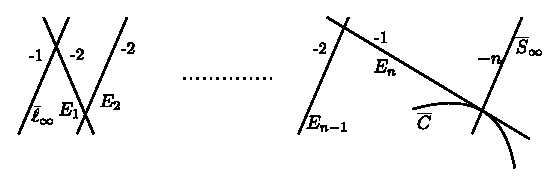
\includegraphics[scale=1.2]{figures/miyansi_fig2.eps}

\bigskip
\centerline{\bf(Fig. 2)}
\end{figure}
\noindent
where\pageoriginale\ $d=3n+1 ~(n>0)~$ and $(\bar{C}, E_n)=3$;
\begin{figure}[H]
\centering
\includegraphics{figures/miyansi_fig3.eps}

\bigskip
\centerline{\bf(Fig. 3)}
\end{figure}
\noindent
where $d=3n+2(n>0)$ and $(\overline{C}\cdot E_{n+1})=2$.

\subsubsection{}\label{chap3:2.5.2}
Since $(A)_{\infty}|_{F_{0}}=3S_{\infty}+d\ell_{\infty}$ we have:
\begin{align*}
(\overline{\sigma}^{\ast}A) &=
  \overline{C}+3(E_{1}+2E_{2}+\cdots+nE_{n})+D-3\\ 
  & \hspace{1cm}(\overline{S}_{\infty}+E_{1}+2E_{2}+\cdots+nE_{n})
 -d(\overline{\ell}_{\infty}+E_{1}+\cdots+E_{n})\\
 & =\overline{C}-3\overline{S}_{\infty} - d \overline{\sigma}^{\ast}
 (\ell_{\infty})+D, \text{ \ if \ } d=3n\\ 
\text{or} &\quad d=3n+1;\\
(\overline{\sigma}^{\ast}A) & \overline{C}+3(E_{1}+2E_{2}+\cdots+nE_{n})+(3n+2)E_{n+1}+D-3(\overline{S}_{\infty}+E_{1}+\\
&\quad 2E_{2}+\cdots+nE_{n}+(n+1)E_{n+1})-d(\overline{\ell}_{\infty}+E_{1}+\cdots+E_{n+1})\\
&= \overline{C}-3\overline{S}_{\infty}-E_{n+1}-\overline{\sigma}^{\ast}(\ell_{\infty})+D,\text{ if } d=3n+2,
\end{align*}
where $D$ is an effective divisor with support in the union
$\mathscr{E}$ of exceptional curves which arise from the quadratic
transformations with centers at the singular points and their
infinitely near singular points\pageoriginale\ of $C$ in the affine
part $\mathbb{A}^{2}_{k}\subset F_{0}$.

\subsubsection{}\label{chap3:2.5.3}
We may write $(\overline{\sigma}^{\ast}A)$ uniquely in the form
$(\overline{\sigma}^{\ast}A)=\overline{B}-2\overline{Z}$ where
$\overline{B}$ is a divisor whose coefficient at each prime divisor is
$0$ or $1$ and where $\overline{Z}$ is some divisor. If $p\neq 2$,
$\overline{B}$ is {\em the branch locus} of a double covering
$\overline{\rho}:\overline{H}\to \overline{F}$, where $\overline{H}$
is the normalization of $\overline{F}$  in $K$ and $\overline{\rho}$
is the normalization morphism (\cf \cite{4}). In order to write down
$\overline{B}$ we consider the following six cases separately.

\paragraph{}\label{chap3:2.5.3.1}
If $d=6m$ (\iec $d=3n$ with $n=2m$) then we have:
\begin{align*}
\overline{B} &= \overline{C}+\overline{S}_{\infty}+D_{1}\\
\overline{Z} &=
2\overline{S}_{\infty}+3m(\overline{\ell}_{\infty}+E_{1}+\cdots+E_{n})-D_{2}, 
\end{align*}
where $D_{1}$ and $D_{2}$ are the divisors determined uniquely by the
conditions that $D_{1}$ is an effective divisor whose coefficient at
each prime divisor is $0$ or $1$, $D_{2}\geqq 0$, $D_{1}+2D_{2}=D$,
and $\Supp(D_{1})\cup \Supp(D_{2})\subset \mathscr{E}$.

\paragraph{}\label{chap3:2.5.3.2}
If $d=6m+1$ (\iec $d=3n+1$ with $n=2m$) then we have:
\begin{align*}
\overline{B} &=
\overline{C}+\overline{S}_{\infty}+(\overline{\ell}_{\infty}+E_{1}+\cdots+E_{n})+D_{1}\\
\overline{Z} &= 2\overline{S}_{\infty}+(3m+1)(\overline{\ell}_{\infty}+E_{1}+\cdots+E_{n})-D_{2},
\end{align*}
where $D_{1}$ and $D_{2}$ are divisors chosen as in \ref{chap3:2.5.3.1}.

\paragraph{}\label{chap3:2.5.3.3}
If $d=6m+2$ (\iec $d=3n+2$ with $n=2m$) then we have:
\begin{align*}
\overline{B} &= \overline{C}+\overline{S}_{\infty}+E_{n+1}+D_{1}\\
\overline{Z} &=
2\overline{S}_{\infty}+E_{n+1}+(3m+1)(\overline{\ell}_{\infty}+E_{1}+\cdots+E_{n+1})-D_{2}, 
\end{align*}
where\pageoriginale\ $D_{1}$ and $D_{2}$ are divisors chosen as in
\ref{chap3:2.5.3.1}.

\paragraph{}\label{chap3:2.5.3.4}
If $d=6m+3$ (\iec $d=3n$ with $n=2m+1$) then we have:
\begin{align*}
\overline{B} &=
\overline{C}+\overline{S}_{\infty}+(\overline{\ell}_{\infty}+E_{1}+\cdots+E_{n})+D_{1}\\
\overline{Z} &= 2\overline{S}_{\infty}+(3m+2)(\overline{\ell}_{\infty}+E_{1}+\cdots+E_{n})-D_{2},
\end{align*}
where $D_{1}$ and $D_{2}$ are divisors chosen as above.

\paragraph{}\label{chap3:2.5.3.5}
If $d=6m+4$ (\iec $d=3n+1$ with $n=2m+1$) then we have:
\begin{align*}
\overline{B} &= \overline{C}+\overline{S}_{\infty}+D_{1}\\
\overline{Z} &=
2\overline{S}_{\infty}+(3m+2)(\overline{\ell}_{\infty}+E_{1}+\cdots+E_{n})-D_{2}, 
\end{align*}
where $D_{1}$ and $D_{2}$ are divisors chooser as above.

\paragraph{}\label{chap3:2.5.3.6}
If $d=6m+5$ (\iec $d=3n+2$ with $n=2m+1$) then we have:
\begin{align*}
\overline{B} &=
\overline{C}+\overline{S}_{\infty}+(\overline{\ell}_{\infty}+E_{1}+\cdots+E_{n})+D_{1}\\
\overline{Z} &= 2\overline{S}_{\infty}+(3m+3)(\overline{\ell}_{\infty}+E_{1}+\cdots+E_{n+1})-D_{2},
\end{align*}
where $D_{1}$ and $D_{2}$ are divisors chosen as above.

\subsection{}\label{chap3:2.6}
Let $\sigma:F\to \overline{F}$ be the shortest succession of quadratic
transformations of $\overline{F}$ such that if one writes
$((\overline{\sigma}\sigma)^{\ast}A)$ in the form
$((\overline{\sigma}\sigma)^{\ast}A)=B-2Z$ with divisors $B$ and $Z$
uniquely determined as in \ref{chap3:2.5.3}, every irreducible component of
$B$ is a connected component of $\Supp(B)$, \iec $\Supp(B)$ is
nonsingular. Let $H$ be the normalization of $F$ in $K$, and let
$\rho:H\to F$ be the normalization morphism. We have a commutative
diagram below: 
\[
\xymatrix@=1.2cm{
H\ar[d]^{\rho}\ar[r]^{\tau} &
\overline{H}\ar[d]^{\overline{\rho}}\ar[r]^{\overline{\tau}} &
H_{0}\ar[d]^{\rho_{0}}  & \\
F\ar[r]^{\sigma} & \overline{F}\ar[r]^{\overline{\sigma}} &
F_{0}\ar[r]^{p_{2}} & \mathbb{P}^{1}_{k},
}
\]\pageoriginale\ 
where $\tau$ and $\overline{\tau}$ are the canonical morphisms which
make each of squares commutative. The following result is well-known
(\cf \cite{4}):

\subsubsection{}\label{chap3:2.6.1}
\begin{lemma*}
  If $p\neq 2$ then $H$ is a nonsingular projective surface defined over $k$.
\end{lemma*}

\begin{proof}
Let $Q$ be a point of $H$, and let $P:=\rho(Q)$. Let
$\widetilde{\mathscr{O}}:=\mathscr{O}_{Q,H}$ and let
$\mathscr{O}:=\mathscr{O}_{P,F}$. We shall show that
$\widetilde{\mathscr{O}}$ is regular for every $k$-rational point
$Q$. If $(\overline{\sigma}\sigma)(P)$ is not a singular point of $C$,
$(\overline{\tau}\tau)(Q)$ is a simple point of $H_{0}$ (\cf Lemma
\ref{chap3:2.4.1}). Hence $Q$ is a simple point. Consider the case where
$(\overline{\sigma}\sigma)(P)$ is a singular point of $C$. If $P\in
\Supp(B)$, we may write $(\overline{\sigma}\sigma)^{\ast}A=hg^{2}$,
where $h\in \mathscr{O}$ and $g\in k(x,y)$ such that $h=0$ is a local
equation of the irreducible component $B_{1}$ of $B$ on which $P$
lies. Since $B_{1}$ is nonsingular, $h$ with some element $h_{1}$ of
$\mathscr{O}$ form a regular system of parameters of
$\mathscr{O}$. Then $t/g$ and $h_{1}$ form a regular system of
parameters of $\widetilde{\mathscr{O}}$. If $P\not\in \Supp(B)$,
$(\overline{\sigma}\sigma)^{\ast}A=g^{2}u$, where $g\in k(x,y)$ and
$u$ is a unit of $\mathscr{O}$. Then there are two distinct points on
$H$ above $P$, one of which is $Q$. Then $Q$ is a simple point since
$[K:k(x,y)]=2$.  
\end{proof}

\subsubsection{}\label{chap3:2.6.2}
\begin{lemma*}
  Assume that $p=2$. Let $Q$ be a point of $H$, and let
  $P:=\rho(Q)$. Then $Q$ is a simple point if $(1)$
  $(\overline{\sigma}\sigma)(P)$ is not a singular point of $C$ or if
  (2) $(\overline{\sigma}\sigma)(P)=P_{\infty}$ (\cf \ref{chap3:2.5}). 
\end{lemma*}

\begin{proof}
The\pageoriginale\ first case follows from Lemma
\ref{chap3:2.4.1}. Consider the case (2). As in \ref{chap3:2.4.4} we may write
$\varphi(y)=y\varphi_{1}(y)^{2}$ with $d_{1}=\deg_{y}\varphi_{1}(y)$
and $d=2d_{1}+1$. We consider the following three cases separately:
(I) $d_{1}=3m$, (II) $d_{1}=3m+1$ and (III) $d_{1}=3m+2$.
\end{proof}

\noindent
{\bf Case (I):}~$d_{1}=3m$. Then $d=6m+1$. The configuration of
$(\overline{\sigma}\sigma)^{-1}(\ell_{\infty}\cup C\cup S_{\infty})$
is easily obtained from the Figure 2 (where $n=2m$):
\begin{figure}[H]
\centering
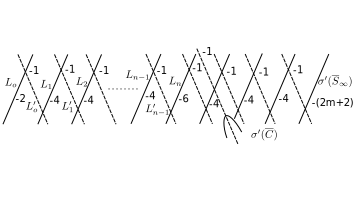
\includegraphics[scale=1.1]{figures/miyansi_fig4.eps}

\bigskip
\centerline{\bf(Fig. 4)}
\end{figure}
\noindent
where the lines represent nonsingular projective rational curves and
the numbers attached to lines are self-intersection multiplicities;
where solid lines (including $\sigma'(\overline{C})$) are contained in
$B$, while the broken lines are not contained in $B$; where
$L_{0}=\sigma'(\overline{\ell}_{\infty})$,
$L'_{0}=\sigma^{-1}(\overline{\ell}_{\infty}\cap E_{1})$,
$L_{i}=\sigma'(E_{i})$ and $L'_{i}=\sigma^{-1}(E_{i}\cap E_{i+1})$ for
$1\leqq i\leqq n$, $L_{n}=\sigma'(E_{n})$ and the remaining unnamed
lines arise from the quadratic transformations with centers at
$E_{n}\cap \overline{S}_{\infty}$ and its infinitely near points. Note
that each broken line has self-intersection multiplicity $-1$ and
meets transversely two irreducible components of $B$. Let $L$ be one
of broken lines, and let $B_{1}$ and $B_{2}$ be irreducible
components\pageoriginale\ of $B$ which meet $L$. Let
$\widehat{\tau}:F\to \widehat{F}$ be the contraction of $L$, and let
$\widehat{P}:=\widehat{\tau}(L)$,
$\widehat{B}_{1}:=\widehat{\tau}(B_{1})$ and
$\widehat{B}_{2}:=\widehat{\tau}(B_{2})$. Let $u=0$ and $v=0$ be local
equations of $\widehat{B}_{1}$ and $\widehat{B}_{2}$ at $\widehat{P}$
on $\widehat{F}$. Let $\widehat{A}$ be the inverse image of $A(x,y)$
on $\widehat{F}$. Then $\widehat{A}=uvTg^{2}$, where $u$, $v$, $T\in
\mathscr{O}_{\widehat{P},\widehat{F}},T(\widehat{P})\neq 0$ and $g\in
k(x,y)$. If $P\in L$ and $P\neq L\cap B_{2}$, then
$(\overline{\sigma}\sigma)^{\ast}A=u_{1}T(vg)^{2}$ with $u_{1}=u/v$,
and $\mathscr{O}_{Q,H}\cong \mathscr{O}_{P,F}[z]/(z^{2}-u_{1}T)$. If
$P=L\cap B_{2}$ then
$(\overline{\sigma}\sigma)^{\ast}A=v_{1}T(ug)^{2}$ with $v_{1}=v/u$,
and $\mathscr{O}_{Q,H}\cong
\mathscr{Q}_{P,F}[z]/(z^{2}-v_{1}T)$. Hence if $P\in L$,
$\mathscr{O}_{Q,H}$ is regular. If $P$ lies on an irreducible
component $B_{1}$ of $B$ then
$(\overline{\sigma}\sigma)^{\ast}A=ug^{2}$, where $g\in k(x,y)$ and
$u=0$ is a local equation of $B_{1}$ at $P$. Hence
$\mathscr{O}_{Q,H}\cong \mathscr{O}_{P,F}[z]/(z^{2}-u)$, and
$\mathscr{O}_{Q,H}$ is regular.

\medskip
\noindent
{\bf Case (II):} $d_{1}=3m+1$. Then $d=6m+3=3n$ with $n=2m+1$. The
configuration of $(\overline{\sigma}\sigma)^{-1}(\ell_{\infty}\cup
C\cup S_{\infty})$ obtained from the Figure 1 is:
\begin{figure}[H]
\centering
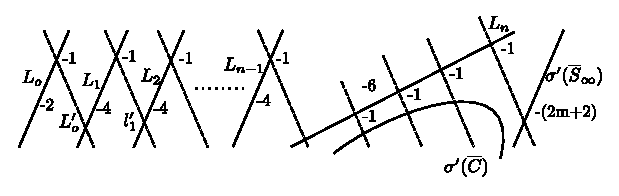
\includegraphics[scale=1.1]{figures/miyansi_fig5.eps}

\bigskip
\centerline{\bf(Fig. 5)}
\end{figure}
\noindent
where we use the same notation as in the Figure 4. Here, note again
that each broken line has self-intersection multiplicity $-1$ and
meets transversely two irreducible components of $B$. We can use the
same argument as in the case (I) to show that $\mathscr{O}_{Q,H}$ is
regular.

\medskip
\noindent
{\bf Case (III):} $d_{1}=3m+2$.\pageoriginale\ Then $d=6m+5=3n+2$ with
$n=2m+1$. The 
configuration of $(\overline{\sigma}\sigma)^{-1}(\ell_{\infty}\cup
C\cup S_{\infty})$ obtained from the Figure 3 is:
\begin{figure}[H]
\centering
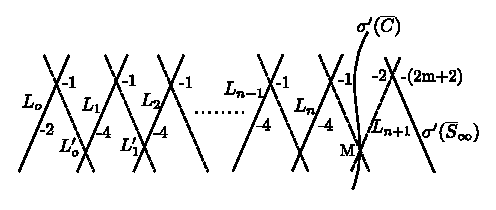
\includegraphics[scale=1.2]{figures/miyansi_fig6.eps}

\bigskip
\centerline{\bf(Fig. 6)}
\end{figure}
\noindent
where $L_{n+1}=\sigma'(E_{n+1})$. Here all broken lines except
$L_{n+1}$ have self-intersection multiplicities $-1$ and meet
transversely two irreducible components of $B$. Thus, if $P\not\in
L_{n+1}$ we can apply the argument in the case (I) to show that
$\mathscr{O}_{Q,H}$ is regular. Consider the case where $P\in
L_{n+1}$. Let $\widehat{\tau}:F\to \widehat{F}$ be the contraction of
$M$ and $L_{n+1}$, and let $\widehat{E}_{n}:=\widehat{\tau}(L_{n})$,
$\widehat{C}:=\widehat{\tau}(\sigma'(\overline{C}))$ and
$\widehat{S}_{\infty}:=\widehat{\tau}(\sigma'(\overline{S}_{\infty}))$. Let
$u=0$ and $v=0$ be local equations of $\widehat{E}_{n}$ and
$\widehat{S}_{\infty}$ respectively at the point
$\widehat{P}:=\widehat{E}_{n}\cap \widehat{S}_{\infty}$ on
$\widehat{F}$. Then the inverse image $\widehat{A}$ of $A(x,y)$ on
$\widehat{F}$ is written in the form
$\widehat{A}=uv(u^{2}+v^{3}T)g^{2}$ with suitable choice of $u$ and
$v$, where $T\in \mathscr{O}_{\widehat{P},\widehat{F}}$,
$T(\widehat{P})\neq 0$ and $g\in k(x,y)$. Then it is easy to show that
$(\overline{\sigma}\sigma)^{\ast}A=u_{2}(u_{2}v+T)(gv^{3})^{2}$ if
$P\in M$ and $P\not\in L_{n+1}$,
$(\overline{\sigma}\sigma)^{\ast}A=(u_{1}+v_{2}T)(gv^{2}u_{1})^{2}$ if
$P\in L_{n+1}$ and $P\not\in \sigma'(\overline{S}_{\infty})$, and
$(\overline{\sigma}\sigma)^{\ast}A=v_{1}(1+uv^{3}_{1}T)(gu^{2})^{2}$
if $P=\sigma'(\overline{S}_{\infty})\cap L_{n+1}$, where $u_{1}=u/v$,
$v_{1}=v/u$, $u_{2}=u_{1}/v$ and $v_{2}=v/u_{1}$. Hence
$\mathscr{O}_{Q,H}\cong
\mathscr{O}_{P,F}[z]/(z^{2}+u_{1}+v_{2}T)$\pageoriginale\ if $P\in
L_{n+1}$ and $P\not\in \sigma'(\overline{S}_{\infty})$, and
$\mathscr{O}_{Q,H}\cong
\mathscr{O}_{P,F}[z]/(z^{2}+v_{1}(1+uv^{3}_{1}T))$ if
$P=\sigma'(\overline{S}_{\infty})\cap L_{n+1}$, whence follows that
$\mathscr{O}_{Q,H}$ is regular.

\subsubsection{}\label{chap3:2.6.3}
In \ref{chap3:2.9.3} below we prove that $H$ is a nonsingular projective
surface defined over $k$.

\subsubsection{}\label{chap3:2.6.4}
In the case where $p\neq 2$ it is easily seen that the configuration
of $(\overline{\sigma}\sigma)^{-1}(\ell_{\infty}\cup C\cup
S_{\infty})$ is the following (\cf \ref{chap3:2.5}):

{\bf Case} $d=6m(m>0)$. Figure 1 with $\overline{\ell}_{\infty}$,
$F_{1},\ldots,E_{n}$ replaces by broken lines.

{\bf Case} $d=6m+1(m>0)$. Figure 4.

{\bf Case} $d=6m+2(m>0)$. Then $d=3n+2$ with $n=2m$.
\begin{figure}[H]
\centering
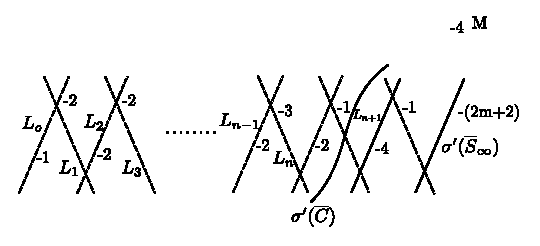
\includegraphics[scale=1]{figures/miyansi_fig7.eps}
\end{figure}

\centerline{\bf(Fig. 7)}

\noindent
where $L_{0}=\sigma'(\overline{\ell}_{\infty})$ and
$L_{i}=\sigma'(E_{i})$ for $1\leqq i\leqq n+1$. 

{\bf Case} $d=6m+3$. Figure 5.

{\bf Case} $d=6m+4$. Then $d=3n+1$ with $n=2m+1$.
\begin{figure}[H]
\centering
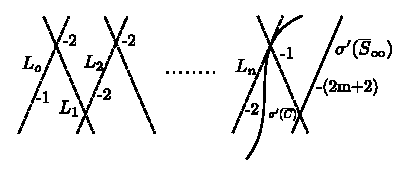
\includegraphics[scale=1.2]{figures/miyansi_fig8.eps}

\bigskip
\centerline{\bf(Fig. 8)}
\end{figure}
\noindent
where\pageoriginale\ $L_{0}=\sigma'(\overline{\ell}_{\infty})$,
$L_{i}=\sigma'(E_{i})$ for $1\leqq i\leqq n$, and
$(L_{n}\cdot\sigma'(\overline{C}))=2$. 

\medskip
\noindent
{\bf Case} $d=6m+5$. Figure 6.

\subsection{}\label{chap3:2.7}
We {\em assume} in this paragraph that $H$ is nonsingular if $p=2$
(\cf \ref{chap3:2.6.3}).

\subsubsection{}\label{chap3:2.7.1}
\begin{lemma*}
  \begin{enumerate}
    \renewcommand{\labelenumi}{\rm(\theenumi)}
  \item Let $D_{1}$ and $D_{2}$ be divisors on $F$. Then
    $(\rho^{\ast}(D_{1})\cdot \rho^{\ast}(D_{2}))=2(D_{1}\cdot D_{2})$.
    
  \item Let $D$ be an irreducible component of $B$. Then
    $\rho^{\ast}(D)=2\Delta$, where $\Delta$ is a nonsingular curve. If
    $D\cong \mathbb{P}^{1}_{k}$, so is $\Delta$.
    
  \item Assume that $p\neq 2$. Let $D$ be a curve on $F$ such that
    $D\cong \mathbb{P}^{1}_{k}$ and $D\not\subset \Supp (B)$.
    \begin{enumerate}
      \renewcommand{\theenumii}{\roman{enumii}}
      \renewcommand{\labelenumii}{\rm(\theenumii)}
    \item If $D\cap \Supp(B)=\phi$ then $\rho^{\ast}(D)=D_{1}+D_{2}$ where
      $D_{1}\cong D_{2}\cong \mathbb{P}^{1}_{k}$, $D_{1}\cap D_{2}=\phi$
      and $(D^{2}_{1})=(D^{2}_{2})=(D^{2})$.
      
    \item If $D$ meets exactly two irreducible components $B_{1}$ and
      $B_{2}$ of $B$ transversely and if $D\cap B_{1}\neq D\cap B_{2}$
      then $\rho^{-1}(D)$ is irreducible and isomorphic to
      $\mathbb{P}^{1}_{k}$.
      
    \item Let $D=L_{n}$ in the Figure $8$. Then
      $\rho^{\ast}(D)=D_{1}+D_{2}$, where $D_{1}\cong D_{2}\cong
      \mathbb{P}^{1}_{k}$, $(D^{2}_{1})=(D^{2}_{2})=-3$ and $(D_{1}\cdot
      D_{2})=1$. 
    \end{enumerate}
  \end{enumerate}
\end{lemma*}

\begin{proof}
(1) and (2) are well-known (\cf \cite{4}) and easy to prove. (3) (i):
  $\rho^{-1}(D)$ is an unramified covering of $D\cong
  \mathbb{P}^{1}_{k}$ of degree $2$. Since $p\neq 2$ and $D$ is simply
  connected, we have $\rho^{\ast}(D)=D_{1}+D_{2}$ with $D_{1}\cong
  D_{2}\cong \mathbb{P}^{1}_{k}$ and $D_{1}\cap D_{2}=\phi$. (ii): Let
  $\rho^{\ast}(B_{1})=2\Delta_{1}$ and
  $\rho^{\ast}(B_{2})=2\Delta_{2}$. Then $\Delta_{1}\cong
  \Delta_{2}\cong \mathbb{P}^{1}_{k}$. Since $(\rho^{\ast}(D)\cdot
  \Delta_{1})=(\rho^{\ast}(D)\cdot \Delta_{2})=1$ and since every
  point except $D\cap B_{1}$ and $D\cap B_{2}$ is not branched, we
  know that $\rho^{-1}(D)\cap \Delta_{1}$ and $\rho^{-1}(D)\cap
  \Delta_{2}$ are simple points of $\rho^{-1}(D)$,\pageoriginale\ and that
  $\rho^{-1}(D)$ is a nonsingular irreducible curve. Then, by
  Hurwitz's formula, $\rho^{-1}(D)$ is isomorphic to
  $\mathbb{P}^{1}_{k}$. (iii): Let $P:=L_{n}\cap
  \sigma'(\overline{C})$. By the quadratic transformations
  $\widehat{\sigma}$ with centers at $P$ and a point of
  $\sigma'(\overline{C})$ infinitely near $P$ we have the following
  configuration: 
\begin{figure}[H]
\centering
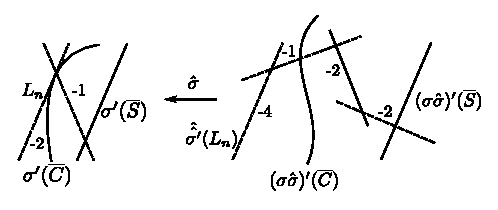
\includegraphics[scale=1.2]{figures/miyansi_fig9.eps}
\end{figure}
\noindent
This implies that $\rho^{\ast}(L_{n})=D_{1}+D_{2}$, where $D_{1}\cong
D_{2}\cong \mathbb{P}^{1}_{k}$. On the other hand, \ref{chap3:2.5.3.5}
implies that $\overline{\sigma}^{\ast}A=u(v+u^{3}T)g^{2}$, where $u$,
$v$, $T\in\mathscr{O}_{\overline{P},\overline{F}}$ with
$\overline{P}:=\overline{S}_{\infty}\cap \overline{C}$,
$T(\overline{P})\neq 0$, $g\in k(x,y)$ and where $u=0$ and $v=0$ are
local equations of $\overline{S}_{\infty}$ and $E_{n}$. Then
$(\overline{\sigma}\sigma)^{\ast}A=(v_{1}+u^{2}T)(gu)^{2}$ locally at
$P$, where $v_{1}=v/u$; and $\mathscr{O}_{Q,H}\cong
\mathscr{O}_{P,F}[z]/(z^{2}-(v_{1}+u^{2}T))$ with
$Q=\rho^{-1}(P)$. Since $L_{n}$ is defined by $v_{1}=0$,
$\rho^{-1}(L_{n})$ is defined by $z^{2}=u^{2}T$. Thus, $(D_{1}\cdot
D_{2})=1$. Since $(D^{2}_{1})=(D^{2}_{2})$ and
$(\rho^{\ast}(L_{n})^{2})=-4$, we have
$(D^{2}_{1})=(D^{2}_{2})=-3$.
\end{proof}


\subsubsection{}\label{chap3:2.7.2}
Let $q:=(p_{2}\overline{\sigma}\sigma\rho):H\to \mathbb{P}^{1}_{k}$,
$\widetilde{C}:=\sigma'(\overline{C})$ and
$\widetilde{S}_{\infty}:=\sigma'(\overline{S}_{\infty})$. Since
$\overline{C}$, $\overline{S}_{\infty}\subset \Supp(\overline{B})$ we
have $\widetilde{C}$, $\widetilde{S}_{\infty}\subset \Supp(B)$. Hence
$\rho^{-1}(\widetilde{C})=2\Gamma$ and
$\rho^{-1}(\widetilde{S}_{\infty})=2\Sigma_{\infty}$ with nonsingular
curves $\Gamma$ and $\Sigma_{\infty}$ on $H$ (\cf \ref{chap3:2.7.1},
(2)). We have then the following:

\begin{lemma*}
Assume that $H$ is nonsingular if $p=2$. Then $q:H\to
\mathbb{P}^{1}_{k}$\pageoriginale\ is an elliptic or quasi-elliptic
fibration with regular cross-section $\Sigma_{\infty}$. The fibration
$q$ is elliptic if $p\neq 2$, $3$; and $q$ is quasi-elliptic if $p=2$
or $3$. Moreover we have:
\begin{enumerate}
\renewcommand{\labelenumi}{\rm(\theenumi)}
\item If $p=3$, $\Gamma$ is the locus of movable singular points of
  $q$.

\item If $p=2$, let $S_{0}$ be the cross-section of $\mathscr{F}$
  defined by $x=0$, and let
  $\Delta:=\rho^{-1}((\overline{\sigma}\sigma)'S_{0})$. Then $\Delta$
  is the locus of movable singular points of $q$.
\end{enumerate}
\end{lemma*}

\begin{proof}
Let $\ell$ be a general member of $\mathscr{F}$, and let
$\widetilde{\ell}=(\overline{\sigma}\sigma)'(\ell)$. Since
$(\widetilde{\ell}\cdot \widetilde{S}_{\infty})=1$ we have
$(\rho^{\ast}(\widetilde{\ell})\cdot \Sigma_{\infty})=1$ which implies
that $\rho^{-1}(\widetilde{\ell})$ is irreducible and
$\rho^{-1}(\widetilde{\ell})\cap \Sigma_{\infty}$ is a simple point of
$\rho^{-1}(\widetilde{\ell})$. Since
$\rho^{-1}(\widetilde{\ell})-\rho^{-1}(\widetilde{\ell})\cap
\Sigma_{\infty}$ is isomorphic to a curve
$t^{2}=x^{3}+\varphi(\alpha)$ for some $\alpha\in k$,
$p_{a}(\rho^{-1}(\widetilde{\ell}))=1$. Thus $q$ is an elliptic or
quasi-elliptic fibration with regular cross-section
$\Sigma_{\infty}$. $\rho^{-1}(\widetilde{\ell})$ has a unique singular
point $(t=0,x=-\varphi(\alpha)^{1/3})$ if $p=3$;
$(t=\varphi(\alpha)^{1/2},x=0)$. Thus, $q$ is quasi-elliptic if $p=2$
or $3$; and $\Gamma$ is the locus of movable singular points of $q$ if
$p=3$, and $\Delta$ is the locus of movable singular points of $q$ if
$p=2$. (It will be easy to see that $\Delta$ is irreducible).
\end{proof}

\subsubsection{}\label{chap3:2.7.3}
Let $q^{-1}(\infty)$ be the fiber of $q$ corresponding to
$y=\infty$. To illustrate $q^{-1}(\infty)\cup \Sigma_{\infty}$ we
shall define {\em the weighted graph of $q^{-1}(\infty)\cup
  \Sigma_{\infty}$} in the following way: Assign a vertex $\circ$ (or $\circ$,
\resp) to each irreducible component $T$ of
$q^{-1}(\infty)\cup\Sigma_{\infty}$ such that $\rho(T)\not\subset
\Supp(B)$ (or $\rho(T)\subset \Supp(B)$, \resp); the weight is
$(T^{2})$; join two vertices by a single edge like $\xymatrix{
  \ar@{o-o}[r] & }$ (or a double edge like $\xymatrix{
  \ar@{o=o}[r] & }$) if the corresponding irreducible components meet
each other transversely\pageoriginale\ in one point (or, touch in one
point with multiplicity 2, \resp). By virtue of \ref{chap3:2.6.4} and
\ref{chap3:2.7.1} we have the following weighted graphs of
$q^{-1}(\infty)\cup \Sigma_{\infty}$ when $p\neq 2$:

\medskip
\noindent
{\bf Case} $d=6m(m>0)$ and $p\neq 3$.
\begin{figure}[H]
\centering
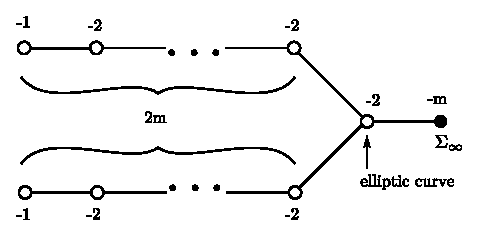
\includegraphics{figures/miyansi_fig10.eps}

\bigskip
\centerline{\bf(Fig. 9)}
\end{figure}
\noindent
where all components of $q^{-1}(\infty)\cup \Sigma_{\infty}$ except
one elliptic component are nonsingular projective rational curves; in
the cases given below all components are nonsingular projective
rational curves.

\medskip
\noindent
{\bf Case} $d=6m+1(m>0)$.
\begin{figure}[H]
\centering
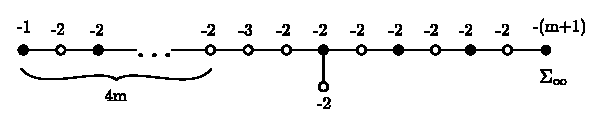
\includegraphics{figures/miyansi_fig11.eps}

\bigskip
\centerline{\bf(Fig. 10)}
\end{figure}


\medskip
\noindent
{\bf Case} $d=6m+2(m>0)$.
\begin{figure}[H]
\centering
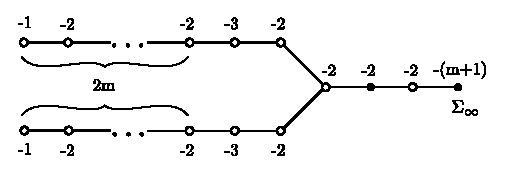
\includegraphics{figures/miyansi_fig12.eps}

\bigskip
\centerline{\bf(Fig. 11)}
\end{figure}
\noindent

\medskip
\noindent
{\bf Case} $d=6m+3(m\geqq 0)$ and $p\neq 3$.
\begin{figure}[H]
\centering
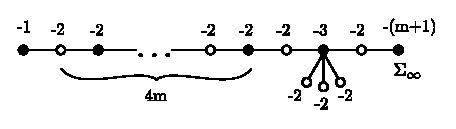
\includegraphics{figures/miyansi_fig12-1.eps}

\bigskip
\centerline{\bf(Fig. 12)}
\end{figure}
\noindent\pageoriginale\

\medskip
\noindent
{\bf Case} $d=6m+4(m\geqq 0)$.
\begin{figure}[H]
\centering
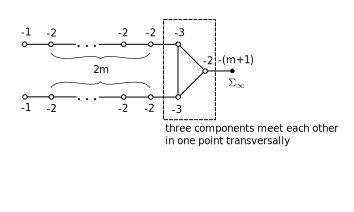
\includegraphics{figures/miyansi_fig13.eps}

\bigskip
\centerline{\bf(Fig. 13)}
\end{figure}
\noindent

\medskip
\noindent
{\bf Case} $d=6m+5(m\geqq 0)$
\begin{figure}[H]
\centering
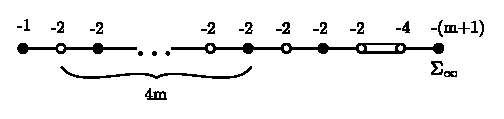
\includegraphics{figures/miyansi_fig14.eps}

\bigskip
\centerline{\bf(Fig. 14)}
\end{figure}
\noindent

\subsubsection{}\label{chap3:2.7.4}
\begin{lemma*}
  Assume that $p=2$ and $H$ is nonsingular. Then the weighted graph of
  $q^{-1}(\infty)\cup \Sigma_{\infty}$ is given as follows:
  \begin{quote}
    {\rm\bf Case} $d=6m+1(m>0)$. {\rm\bf Figure 10.}
    
    {\rm\bf Case} $d=6m+3(m\geqq 0)$. {\rm\bf Figure 12.}
    
    {\rm\bf Case} $d=6m+5(m\geqq 0)$. {\rm\bf Figure 14.}
  \end{quote}
\end{lemma*}

\begin{proof}
Lemma follows from \ref{chap3:2.3.4} and \ref{chap3:2.7.2}. We shall only indicate
how to use these results. {\bf Case} $d=6m+1$. With the notations of
\ref{chap3:2.6.2}, for all solid lines $L$, $\rho^{-1}(L)=2\widetilde{L}$
with $\widetilde{L}\cong \mathbb{P}^{1}_{k}$ and
$2(\widetilde{L}^{2})=(L^{2})$; for all broken lines $L$ with
$(L^{2})=-1$, $\widetilde{L}:=\rho^{-1}(L)$ is irreducible. Thus the
weighted graph of $q^{-1}(\infty)\cup \Sigma_{\infty}$ is: 
\begin{figure}[H]
\centering
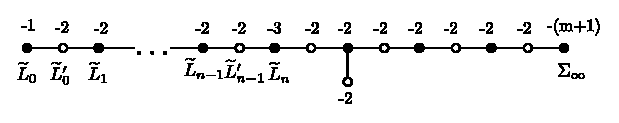
\includegraphics{figures/miyansi_fig15.eps}
\end{figure}
\noindent\pageoriginale\
where $\bullet$ represents a nonsingular projective rational
curve. Let $\nu$ be the contraction of $\widetilde{L}_{0}$. If
$\nu(\widetilde{L}'_{0})\neq \mathbb{P}^{1}_{k}$,
$\nu(q^{-1}(\infty))$ would be a reducible fiber of a relatively
minimal quasi-elliptic fibration. Then, by lemma \ref{chap3:2.3.4},
$\nu(\widetilde{L}'_{0})\cong\mathbb{P}^{1}_{k}$, which is a
contradiction. Hence $\nu(\widetilde{L}'_{0})\cong\mathbb{P}^{1}_{k}$
and $(\nu(\widetilde{L}'_{0})^{2})=-1$, whence
$\nu(\widetilde{L}'_{0})$ is contractible. Repeating this argument for
$\widetilde{L}_{0}$, $\widetilde{L}'_{0},\ldots,\widetilde{L}'_{n-1}$
we can see that they are all isomorphic to $\mathbb{P}^{1}_{k}$. Let
$\pi$ be the contraction of
$\widetilde{L}_{0},\ldots,\widetilde{L}'_{n-1}$. Then
$\pi(\widetilde{L}_{n})\cong \mathbb{P}^{1}_{k}$ and
$(\pi(\widetilde{L}_{n})^{2})=-2$. Hence $\pi(q^{-1}(\infty))$ is a
reducible fiber of a relatively minimal quasi-elliptic fibration. Then
the remaining components are all isomorphic to $\mathbb{P}^{1}_{k}$ by
virtue of \ref{chap3:2.3.4}. The {\bf case} $d=6m+3$ can be treated in the
same fashion as above. {\bf Case} $d=6m+5$. The weighted graph of
$q^{-1}(\infty)\cup\Sigma_{\infty}$ is:
\begin{figure}[H]
\centering
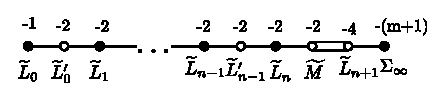
\includegraphics{figures/miyansi_fig16.eps}
\end{figure}
\noindent
where represents a curve isomorphic to $\mathbb{P}^{1}_{k}$;
$\widetilde{L}_{n+1}:=\rho^{-1}(L_{n+1})$ is reduced (and irreducible)
because $(\widetilde{L}_{n+1}\cdot\Sigma_{\infty})=1$;
$\widetilde{M}:=\rho^{-1}(M)$ touches $\widetilde{L}_{n+1}$ in one
point with multiplicity $2$. The foregoing argument shows that
$\widetilde{L}_{0},\ldots,\widetilde{L}_{n}$, $\widetilde{M}$ are
isomorphic to $\mathbb{P}^{1}_{k}$ and contractible. Let $\pi$ be the
contraction of those curves. Then $\pi(\widetilde{L}_{n+1})$ is an
irreducible member of a relatively minimal quasi-elliptic
fibration. Hence $\pi(\widetilde{L}_{n+1})$ has one cusp, and
$\widetilde{L}_{n+1}$ is a\pageoriginale\ nonsingular projective
rational curve.
\end{proof}

\subsubsection{}\label{chap3:2.7.5}
By contracting all possible exceptional components of
$q^{-1}(\infty)$, the image of $q^{-1}(\infty)\cup\Sigma_{\infty}$ has
the following weighted graph (or configuration); the type of a
singular fiber according to \v{S}afarevi\v{c} \cite{51} is also given:

\medskip
\noindent
{\bf Case} $d=6m$. \qquad $o$ (elliptic curve)

\medskip
\noindent
{\bf Case} $d=6m+1$.
\begin{figure}[H]
\centering
\includegraphics{figures/miyansi_fig17.eps}
\end{figure}


\noindent
{\bf Case} $d=6m+2$.
\begin{figure}[H]
\centering
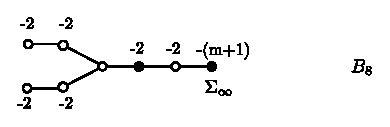
\includegraphics{figures/miyansi_fig18.eps}
\end{figure}

\noindent
{\bf Case} $d=6m+3$.
\begin{figure}[H]
\centering
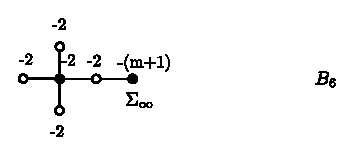
\includegraphics{figures/miyansi_fig19.eps}
\end{figure}

\noindent
{\bf Case} $d=6m+4$.\pageoriginale\
\begin{figure}[H]
\centering
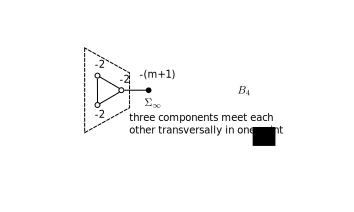
\includegraphics{figures/miyansi_fig20.eps}
\end{figure}

\noindent
{\bf Case} $d=6m+5$.
\begin{figure}[H]
\centering
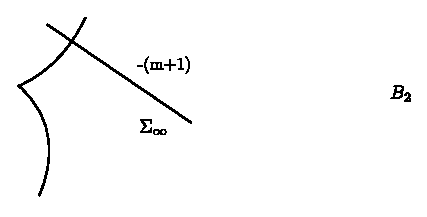
\includegraphics{figures/miyansi_fig21.eps}
\end{figure}

\subsection{}\label{chap3:2.8}
We shall proceed to a proof of Theorem \ref{chap3:2.1.1}. It is easy to
see that $K$ is rational over $k$ if $d=0$, $1$ or $2$. We shall
therefore assume that $d>3$.

\subsubsection{}\label{chap3:2.8.1}
Consider reducible fibers of $q:H\to \mathbb{P}^{1}_{k}$ other than
$q^{-1}(\infty)$. Such a fiber
$q^{-1}(\alpha):=(\overline{\sigma}\sigma\rho)^{-1}(\ell_{\alpha})$
has more than two reducible components, and $\ell_{\alpha}\cap C$ is a
singular point of $C$, whence $\varphi'(\alpha)=0$. Conversely, for a
root $\alpha$ of $\varphi'(y)=0$, $q^{-1}(\alpha)$ is a reducible
fiber of $q$ (\cf \ref{chap3:2.5}). Let $\alpha$ be a root of
$\varphi'(y)=0$, let $P:=(x=-\varphi(\alpha)^{1/3}.y=\alpha)$ be the
corresponding singular point of $C$, and let
$e=v_{\alpha}(\varphi(y)-\varphi(\alpha))$. The condition (1) of
Theorem \ref{chap3:2.1.1} tells us that $e=2$, $3$, $4$ or $5$, while the
condition (2) asserts that the case $e=3$ can be reduced to the case
$e=4$ or $5$ by a\pageoriginale\ birational transformation
$(t,x,y)\mapsto (t,x+a^{1/3}(y-\alpha),y)$ which is biregular at
$P$. $P$ is then a cuspidal singular point of $C$ with multiplicity
$(2,1,\ldots)$ if $e=2$; $(3,1,\ldots)$ if $e=4$; $(3,2,1,\ldots)$ if
$e=5$. Now the weighted graph of $q^{-1}(\alpha)\cup \Sigma_{\infty}$
is given as follows by making a similar argument as in \ref{chap3:2.5}:

\medskip
\noindent
{\bf Case} $e=2$.
\begin{figure}[H]
\centering
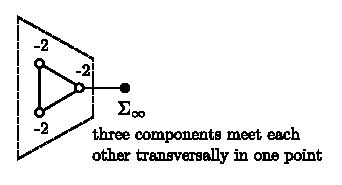
\includegraphics{figures/miyansi_fig22.eps}
\end{figure}
(cf. 2.7.1, (3) (iii))

\noindent
{\bf Case} $e=4$.
\begin{figure}[H]
\centering
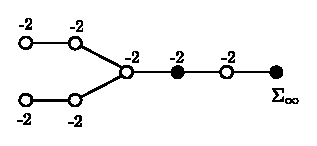
\includegraphics{figures/miyansi_fig23.eps}
\end{figure}

\noindent
{\bf Case} $e=5$.
\begin{figure}[H]
\centering
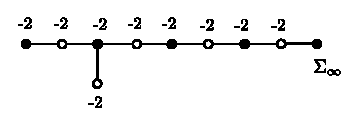
\includegraphics{figures/miyansi_fig24.eps}
\end{figure}
Notice that $q^{-1}(\alpha)$ contains no exceptional components. The
type of a singular fiber according to \v{S}afarevi\v{c} \cite{51} is
$B_{4}$ if $e=2$; $B_{8}$ if $e=4$; $B_{10}$ if $e=5$.

\subsubsection{}\label{chap3:2.8.2}
As\pageoriginale\ shown in \ref{chap3:2.8.1}, $q^{-1}(\infty)$ is the only
singular fiber in the fibration $q$, which contains exceptional
components. By a contraction $\widehat{\tau}:H\to \widehat{H}$ of all
exceptional components in $q^{-1}(\infty)$ we get a relatively minimal
quasi-elliptic surface $\widehat{q}:\widehat{H}\to \mathbb{P}^{1}_{k}$
with $\widehat{q}\widehat{\tau}=q$, for which
$\widehat{\Sigma}_{\infty}:=\widehat{\tau}(\Sigma_{\infty})$ is a
regular cross-section with
$(\widehat{\Sigma}^{2}_{\infty})=-(m+1)$. (Since we are dealing with
the case $p=3$, look at only the cases $d=6m+1$, $d=6m+2$, $d=6m+4$
and $d=6m+5$). Now, Theorem 2 follows immediately from \ref{chap3:2.2},
\ref{chap3:2.3.2} and \ref{chap3:2.3.3}.

\subsection{}\label{chap3:2.9}
We shall now prove Theorem \ref{chap3:2.1.2}. The first assertion follows
from \ref{chap3:2.2}. So, we shall prove the second assertion. To be in
accordance with the notations in the paragraphs \ref{chap3:2.4} $\sim$
\ref{chap3:2.7} we start with an equation $t^{2}=x^{3}+\varphi(y)$, where
$\varphi(y)=y\varphi_{1}(y)^{2}$, $d:=\deg_{y}\varphi$ and
$d_{1}:=\deg_{y}\varphi_{1}$. Hence $d=2d_{1}+1$. We have only to
consider the cases $d=6m+1$, $d=6m+3$ and $d=6m+5$. Moreover, since
$K$ is easily seen to be rational over $k$ if $d=1$ we assume that
$d\geqq 3$.

\subsubsection{}\label{chap3:2.9.1}
Write
$$
\varphi_{1}(y)=a(y-\alpha_{1})^{r_{1}}\ldots(y-\alpha_{s})^{r_{s}},
$$
where $a\in k^{\ast}$, $\alpha_{i}\in k$, and $\alpha_{i}$'s are
mutually distinct. The assumption in Theorem \ref{chap3:2.1.2} implies
that $r_{i}\leqq 2$ for every $i$. For if $r_{i}\geqq 3$,
$\varphi(y+\alpha_{i})$ starts with a term of degree $\geqq 6$. The
singular points of $C$ lying on the affine part $F_{0}-(x=\infty)\cup
(y=\infty)$ are given by $(x=0,y=\alpha_{i})$ for $1\leqq i\leqq
s$. Let $P:=(t=0,x=0,y=\alpha)$ with $\varphi_{1}(\alpha)=0$. By a
birational transformation $(t,x,y)\mapsto (t,x,y+\alpha)$ which is
biregular at $P$, $H_{0}$ is a hyper surface in $\mathbb{A}^{3}_{k}$
defined locally at\pageoriginale\ $P$ by one of the following
equations:
\begin{itemize}
\item[(i)] $t^{2}=x^{3}+y^{2}\delta(y)$\quad if\quad $\alpha\neq
  0$ \ and \ $r=1$

\item[(ii)] $t^{2}=x^{3}+y^{3}\delta(y)$\quad if\quad $\alpha=
  0$ \ and \ $r=1$

\item[(iii)] $t^{2}=x^{3}+y^{4}\delta(y)$\quad if\quad $\alpha\neq
  0$ \ and \ $r=2$

\item[(iv)] $t^{2}=x^{3}+y^{5}\delta(y)$\quad if\quad $\alpha=
  0$ \ and \ $r=2$,
\end{itemize}
where $\delta(y)\in k[y]$, $\delta(0)\neq 0$, and
$\delta(y)y^{2r+\epsilon}=\varphi(y+\alpha)$ with $\epsilon=0$ or $1$
according as $\alpha\neq 0$ or $\alpha=0$.

\subsubsection{}\label{chap3:2.9.2}
Now write
$$
\delta(y)=a_{0}+a_{1}y+a_{2}y^{2}+a_{3}y^{3}+\cdots\quad\text{with}\quad
a_{0}\neq 0.
$$
The case (i) above is now reduced to the case (ii) or (iv) by a
birational transformation $(t,x,y)\mapsto
(t+a_{0}^{1/2}y+a^{1/2}_{2}y^{2},x,y)$ which is biregular at
$P$. Namely, if $a_{1}\neq 0$ we have the case (ii); if $a_{1}=0$ and
$a_{3}\neq 0$ we have case (iv). (Note that $a_{1}=a_{3}=0$ does not
occur). Similarly, the case (iii) is reduced to the case (iv). Thus,
in order to look into the singularity of $P$, we have only to consider
the cases (ii) and (iv).

\subsubsection{}\label{chap3:2.9.3}
Let $\ell_{0}$ be the member of $\mathscr{F}$ passing through the
point $(x=0,y=\alpha)$. The configuration of
$(\overline{\sigma}\sigma)^{-1}(\ell_{0}\cup C\cup S_{\infty})$ is
given as follows:

\medskip
\noindent
{\bf Case (ii):}
\begin{figure}[H]
\centering
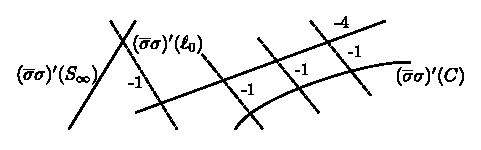
\includegraphics{figures/miyansi_fig25.eps}
\end{figure}

\noindent
{\bf Case (iv):}\pageoriginale\
\begin{figure}[H]
\centering
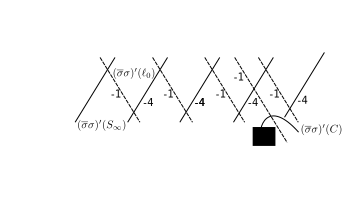
\includegraphics{figures/miyansi_fig26.eps}
\end{figure}
The meanings of solid or broken lines are the same as in
\ref{chap3:2.6.2}. By the same argument as in \ref{chap3:2.6.2} (especially the
proof of Case (I) there) we can show:

\begin{lemma*}
Let $Q$ be a point on $H$ such that
$(\overline{\sigma}\sigma\rho)(Q)=(x=0,y=\alpha)$. Then $Q$ is a
simple point. Therefore $H$ is nonsingular.
\end{lemma*}

\subsubsection{}\label{chap3:2.9.4}
Now, the weighted graph of
$q^{-1}(\alpha):=\rho^{-1}((\overline{\sigma}\sigma)'(\ell_{0}))$ is
given as follows:

\medskip
\noindent
{\bf Case (ii).}
\begin{figure}[H]
\centering
\includegraphics{figures/miyansi_fig27.eps}
\end{figure}

\noindent
{\bf Case (iv).}
\begin{figure}[H]
\centering
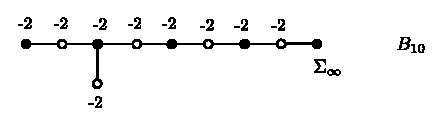
\includegraphics{figures/miyansi_fig28.eps}
\end{figure}
\noindent
(For the proof, see \ref{chap3:2.7.4}). Thus, $q^{-1}(\alpha)$ contains no
exceptional components. The proof of Theorem \ref{chap3:2.1.2} is now
completed as in \ref{chap3:2.8.2}. (Consider only the cases $d=6m+1$,
$d=6m+3$ and $d=6m+5$). 

\section[Unirational surface with.....]{Unirational surface with a pencil of quasi-hyper-elliptic
  curves of genus $2$ (in characteristic
  $5$)}\label{chap3:chap3-sec3}\pageoriginale\

\subsection{}\label{chap3:3.1}
Throughout this section the ground field $k$ is assumed to be an
algebraically closed field of characteristic $5$. A nonsingular
projective surface $X$ is said to have {\em a pencil of
  quasi-hyper-elliptic curves of genus} $2$ if there exists a
surjective morphism $f:X\to C$ from $X$ to a nonsingular projective
curve $C$ such that almost all fibers of $f$ are irreducible singular
curves of arithmetic genus $2$. {\em We assume that $f:X\to C$ has a
  rational cross-section}. The purpose of this section is to prove the
following: 

\begin{theorem*}
Let $k$ be an algebraically closed field of characteristic $5$. Then
any unirational surface $X$ with a pencil of quasi-hyperelliptic\break 
curves of genus 2 defined over $k$ is birationally equivalent to a
hyper surface in $\mathbb{A}^{3}_{k}:t^{2}=x^{5}+\varphi(y)$ with
$\varphi(y)\in k[y]$, provided $X$ has a rational
cross-section. Conversely, let $K:=k(t,x,y)$ be the function field of
an affine hyper surface of the above type. Assume that $\varphi(y)$
satisfies the conditions:
\begin{enumerate}
\renewcommand{\labelenumi}{\rm(\theenumi)}
\item $\varphi(y)$ has no terms of degree multiples of $5$,

\item every root of $\varphi'(y)\left(=\dfrac{d\varphi}{dy}\right)$ is at most a
  double point.
\end{enumerate}
Let $d:=\deg_{y}\varphi$, $m:=[d/10]$ and $X$ the nonsingular minimal
model if $K$ is not rational. Then the structure of $X$ is determined
as follows:
\end{theorem*}

\medskip
\noindent
{\bf Case} $m=0$.\pageoriginale\
\begin{center}
%\tabcolsep=.4cm
\begin{tabular}{|c|c|c|c|c|c|c|c|c|}
\hline
$d$ & 1 & 2 & 3 & 4 & 6 & 7 & 8 & 9\\
\hline
$p_{a}(X)$ & 0 & 0 & 0 & 1 & 1 & 2 & 2 & 2\\
\hline
$(K^{2}_{X})$ & & & & 0 & 0 & 1 & 1 & 1\\
\hline
\multirow{3}{*}{structure} & \multicolumn{3}{c|}{rational} &
\multicolumn{2}{l|}{unirational} & \multicolumn{3}{l|}{unirational}\\ 
 & \multicolumn{3}{c|}{surface} & \multicolumn{2}{l|}{K3-surface} &
\multicolumn{3}{l|}{surface of}\\
& \multicolumn{3}{c|}{} & \multicolumn{2}{c|}{} &\multicolumn{3}{l|}{general type}\\
\hline
\end{tabular}
\end{center}

\medskip

\noindent
{\bf Case} $m>0$.
\begin{center}
{\fontsize{9pt}{11pt}\selectfont
\tabcolsep=2.5pt
\begin{tabular}{|>{$}c<{$}|>{$}c<{$}|>{$}c<{$}|>{$}c<{$}|>{$}c<{$}|>{$}c<{$}|>{$}c<{$}|>{$}c<{$}|>{$}c<{$}|}
\hline
d & 10m+1 & 10m+2 & 10m+3 & 10m+4 & 10m+6 & 10m+7 & 10m+8 & 10m+9\\
\hline
p_{a}(X) & 4m & 4m & 4m & 4m+1 & 4m+1 & 4m+2 & 4m+2 & 4m+2\\
\hline
(K^{2}_{X}) & 8m-4 & 8m-4 & 8m-3 & 8m-2 & 8m-2 & 8m & 8m & 8m\\
\hline
\end{tabular}}\relax
\end{center}
{\em The surface $X$ is then a unirational surface of general type.}

A proof which is given in the subsequent paragraphs will be not more
than a sketchy one, as the arguments are similar to the ones in the
previous section.

\subsection{}\label{chap3:3.2}
Let $f:X\to C$ be as in \ref{chap3:3.1}. Let $\mathscr{R}$ be the function
field of $C$ over $k$ and let $X_{\mathscr{R}}$ be the generic fiber
of $f$. Then $X_{\mathscr{R}}$ is an irreducible normal projective
curve with $p_{a}(X_{\mathscr{R}})=2$. Let $\mathscr{R}_{s}$ be a
separable algebraic closure of $\mathscr{R}$. by Chevalley [12; Th.\@
  5, p.99], $\foprod{X}{\mathscr{R}_{s}}{\mathscr{R}}$ is a normal
projective curve of arithmetic genus $2$. Hence, every singular point
of $X_{\mathscr{R}}$ is a one-place point and is rational over a
purely inseparable extension of $\mathscr{R}$. If the
geometric\pageoriginale\ genus of $X_{\mathscr{R}}$ equals $1$ then
$X_{\mathscr{R}}$ has a single ordinary cusp of multiplicity $2$ as
its unique singularity. However, this is impossible by virtue of Tate
\cite{55} because the characteristic of $k$ is $5$. Thus the geometric
genus of $X_{\mathscr{R}}$ is $0$ and $X_{\mathscr{R}}$ has either two
ordinary cusps of multiplicity $2$ or a single cuspidal point of
multiplicity $(2,2,1,\ldots)$ as its singularity. We shall see that
the former case does not occur. Indeed, let $Q$ be one of two ordinary
cusps, let $\Gamma$ be the closure of $Q$ in $X$ and let
$f_{\Gamma}:\Gamma\to C$ be the restriction of $f$ onto
$\Gamma$. Since $Q$ is a one-place point of $X_{\mathscr{R}}$,
$f_{\Gamma}$ is a generically one-to-one morphism. Hence $\deg
f_{\Gamma}$ is a power $p^{n}$ of the characteristic $p$ of $k$. For a
point $P$ of $C$ such that $f^{-1}(P)$ meets $\Gamma$ at a simple
point of $\Gamma$, we have $(f^{-1}(P)\cdot \Gamma)=2$ or $3$ because
$f^{-1}(P)\cap \Gamma$ is an ordinary cusp of multiplicity $2$ on
$f^{-1}(P)$. This is a contradiction because $p=5$. Therefore we know
that $X_{\mathscr{R}}$ is an irreducible normal projective curve of
arithmetic genus $2$ and geometric genus $0$ and with a single
cuspidal point of multiplicity $(2,2,1,\ldots)$ as its unique
singularity. This implies that $X_{\mathscr{R}}$, minus the unique
singular point, is a $\mathscr{R}$-form of the affine line
$\mathbb{A}^{1}$ of $\mathscr{R}$-genus $2$. We {\em assume} that
$f:X\to C$ has a rational cross-section, {\em viz.\@}
$X_{\mathscr{R}}$ has a $\mathscr{R}$-rational point. Then, by virtue
of Lemma \ref{chap3:1.5.1}, $X_{\mathscr{R}}$ is
$\mathscr{R}$-birationally equivalent to an affine plane curve:
\begin{equation*}
t^{2}=x^{5}+a\quad\text{with}\quad a\in \mathscr{R}-\mathscr{R}^{5}.\tag{1}
\end{equation*}
The surface $X$ is unirational over $k$ if and only if $C$ is rational
over $k$. Indeed, the ``only if'' part follows from the L\"uroth's
theorem;\pageoriginale\ the ``if'' part holds because
$\foprod{\mathscr{R}^{1/5}}{k(X)}{\mathscr{R}}$ is rational over
$k$. Now {\em assume} that $X$ is unirational over $k$ and write
$\mathscr{R}:=k(y)$. Then $X$ is $k$-birationally equivalent to a
hyper surface in $\mathbb{A}^{3}_{k}$:
\begin{align*}
& t^{2}=x^{5}+\varphi(y)\quad\text{with}\quad \varphi(y)\in k[y],\tag{2}\\
& \text{where } d:=\deg_{y}\varphi\text{ \  is prime to 5.}
\end{align*}
This proves the first assertion in the theorem. Conversely, let
$K:=k(t,x,y)$ be the function field of a hyper surface (2) and let $X$
be a nonsingular projective model of $K$; we denote by $X$ a
nonsingular minimal model of $K$ if $K$ is not rational over $k$. We
may assume without loss of generality that the following conditions
are satisfied:
\begin{itemize}
\item[(i)] $\varphi(y)$ has no terms of degree multiples of $5$.

\item[(ii)] Let $\alpha$ and $\beta(\in k)$ satisfy
  $\varphi'(\alpha)=0$ and $\beta^{5}+\varphi(\alpha)=\sigma$. Then
  $e:=v_{\alpha}(\varphi(y)-\varphi(\alpha))$ satisfies $2\leqq e\leqq
  9$ and $e\neq 5$.
\end{itemize}
Indeed, a birational transformation of the type $(t,x,y)\mapsto
(t,x+\rho(y),y)$ annihilates the terms of degree multiples of $5$ in
$\varphi(y)$. With the notations of (ii), the hyper surface is written
as 
$$
t^{2}=(x-\beta)^{5}+(y-\alpha)^{e}\varphi_{1}(y)\quad\text{with}\quad
\varphi_{1}(\alpha)\neq 0.
$$
If $e\geqq 10$ the degree of $\varphi(y)$ drops by a birational
transformation $(t,x,y)$ $\mapsto (t/(y-\alpha)^{5}$,
$(x-\beta)/(y-\alpha)^{2},y)$. Hence we may assume that $e\leqq 9$. If
$e=5$ a birational transformation $(t,x,y)\mapsto
(t,(x-\beta)+\gamma(y-\alpha),y)$ with $\gamma^{5}=\varphi_{1}(0)$
enables us to assume. $e\geqq 6$. 

\subsection{}\label{chap3:3.3}
Set\pageoriginale\ $A(x,y):=x^{5}+\varphi(y)$. Embed
$\mathbb{A}^{2}_{k}:=\Spec(k[x,y])$ into
$F_{0}:=\mathbb{P}^{1}_{k}\times\mathbb{P}^{1}_{k}$ as the complement
of two lines $(x=\infty)\cup (y=\infty)$ and let $C$ be the curve on
$F_{0}$ defined by $A(x,y)=0$. Let $H_{0}$ be the normalization of
$F_{0}$ in $K:=k(t,x,y)$ and let $\rho_{0}:H_{0}\to F_{0}$ be the
normalization morphism. Then $\rho_{0}$ is a double covering with $C$
contained in the branch locus. We shall look for a de singularization
of $H_{0}$. As is well-known (\cf \ref{chap3:2.5} and \ref{chap3:2.6}), a
de singularization of $H_{0}$ is obtained as follows. Let
$\overline{\sigma}:\overline{F}\to F_{0}$ be the shortest succession
of quadratic transformations with centers at singular points of $C$
such that $\overline{C}:=\overline{\sigma}'(C)$ is nonsingular, let
$\overline{H}$ be the normalization of $\overline{F}$ in $K$ and let
$\overline{\rho}:\overline{H}\to \overline{F}$ be the normalization
morphism. Write $(\overline{\sigma}^{\ast}A)$ in the form:
$$
(\overline{\sigma}^{\ast}A)=\overline{B}-2\overline{Z},
$$
where $\overline{B}$ is a divisor whose coefficient at each prime
divisor is $0$ or $1$ and $\overline{Z}$ is some divisor. Then
$\overline{B}$ is the branch locus of a double covering
$\overline{\rho}:\overline{H}\to \overline{F}$. If $\overline{B}$ is
nonsingular then $\overline{H}$ is nonsingular. If $\overline{B}$ is
singular, let $\sigma:F\to \overline{F}$ be the shortest succession of
quadratic transformations with centers at singular points of
$\Supp(\overline{B})$ such that, if one writes
$((\overline{\sigma}\sigma)^{\ast}A)=B-2Z$ with divisors $B$ and $Z$
as above, $B$ is nonsingular, {\em viz.\@} every irreducible component
of $\Supp(B)$ is a connected component. Let $H$ be the normalization
of $F$ in $K$ and let $\rho:H\to F$ be the normalization
morphism. Then $\rho$ is a double covering with branch locus $B$, and
$H$ is nonsingular. Thus $H$ is a de singularization of $H_{0}$; we
have a commutative diagram 
\[
\xymatrix@R=1.1cm@C=1.2cm{
H\ar[d]^{\rho}\ar[r]^{\tau} &
\overline{H}\ar[d]^{\overline{\rho}}\ar[r]^{\overline{\tau}} &
H_{0}\ar[d]^{\rho_{0}}\\
F\ar[r]^{\sigma} & \overline{F}\ar[r]^{\overline{\sigma}} & F_{0},
}
\]\pageoriginale\
where $\tau$ and $\overline{\tau}$ are the canonical morphisms induced
by the normalizations. Set $\pi:=\sigma\cdot\rho$. The curve
$\overline{B}$ is said to have {\em a negligible singularity} at a
point $P$ if one of the following conditions is satisfied:
\begin{enumerate}
\renewcommand{\labelenumi}{(\theenumi)}
\item $\overline{B}$ is nonsingular at $P$,

\item $P$ is a double point,

\item $P$ is a triple point with at most a double point (not
  necessarily ordinary) infinitely near.
\end{enumerate}

If $\overline{B}$ has only negligible singularities then some
numerical invariants of $H$ are computable at the stage of
$\overline{F}$. Namely we have:

\begin{lemma*}[Artin \cite{4}]
Assume that $\overline{B}$ has only negligible singularities. Then the
following assertions hold true.
\begin{enumerate}
\renewcommand{\labelenumi}{\rm(\theenumi)}
\item $\pi^{\ast}(K_{\overline{F}}+\overline{Z})$ is a canonical
  divisor $K_{H}$ on $H$.

\item
  $p_{a}(H)=2p_{a}(F_{0})+p_{a}(\overline{Z})=p_{a}(\overline{Z})$.

\item $(K^{2}_{H})=2((K_{\overline{F}}+\overline{Z})^{2})$.
\end{enumerate}
\end{lemma*}

\subsection{}\label{chap3:3.4}
We shall look into singular points of the curve $C$ on $F_{0}$. Let
$P:=(x=\beta,y=\alpha)$ be a singular point of $C$ lying on the affine
part $\mathbb{A}^{2}_{k}:F_{0}-(x=\infty)\cup (y=\infty)$. Then
$\varphi'(\alpha)=\beta^{5}+\varphi(\alpha)=0$. Conversely, every root
of $\varphi'(y)=0$ gives rise to a singular point of $C$ lying on
$\mathbb{A}^{2}_{k}$. Let $P:=(x=\beta,y=\alpha)$ be such a singular
point and let
$e:=V_{\alpha}(\varphi(y)-\varphi(\alpha))$.\pageoriginale\ Then $P$ is
a one-place point of $C$, and we have $2\leqq e\leqq 9$ and $e\neq 5$
as we assumed in \ref{chap3:3.2}. Let $D_{P}$ be the contribution by $P$ in
the effective divisor $\overline{\sigma}^{\ast}(C)-\overline{C}$, and
write $D_{P}=D^{(1)}_{P}+2D^{(2)}_{P}$, where $D^{(1)}_{P}\geqq 0$,
$D^{(2)}_{P}\geqq 0$ and every component of $D^{(1)}_{P}$ has
multiplicity $1$. Let $D^{(3)}_{P}$ be the contribution by $P$ in the
effective divisor
$K_{\overline{F}}-\overline{\sigma}^{\ast}(K_{F_{0}})$. In the
  following, we shall compute the values
  $\mu_{P}:=\dfrac{1}{2}(D^{(2)}_{P}\cdot D^{(2)}_{P}-D^{(3)}_{P})$
  and $\nu_{P}:=((D^{(2)}_{P}-D^{(3)}_{P})^{2})$ for each type of a
  singular point $P$ of $C$.

\medskip
\noindent
{\bf Case} $e=2$. Then $P$ has multiplicity $(2,2,1,\ldots)$ and
$\overline{\sigma}^{-1}(P)$ has the configuration
\begin{figure}[H]
\centering
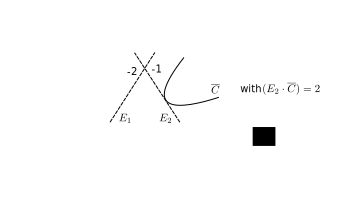
\includegraphics{figures/miyansi_fig30.eps}
\end{figure}
\noindent
(\cf \ref{chap3:2.6.2} for the conventions on the broken lines and solid
curve (or line)). Hence $D_{P}=2E_{1}+4E_{2}$, $D^{(1)}_{P}=0$,
$D^{(2)}_{P}=E_{1}+2E_{2}$ and $D^{(3)}_{P}=E_{1}+2E_{2}$;
$\mu_{P}=\nu_{P}=0$.

\medskip
\noindent
{\bf Case} $e=3$. Then $P$ has multiplicity $(3,2,1,\ldots)$ and
$\overline{\sigma}^{-1}(P)$ has the configuration:
\begin{figure}[H]
\centering
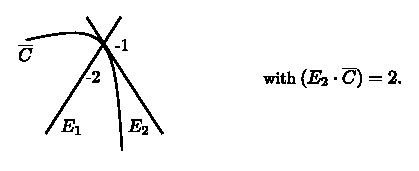
\includegraphics{figures/miyansi_fig31.eps}
\end{figure}
Then\pageoriginale\ we have: $D_{P}=3E_{1}+5E_{2}$,
$D^{(1)}_{P}=E_{1}+E_{2}$, $D^{(2)}_{P}=E_{1}+2E_{2}$,
$D^{(3)}_{P}=E_{1}+2E_{2}$ and $\mu_{P}=\nu_{P}=0$.

\medskip
\noindent
{\bf Case} $e=4$. $P$ has multiplicity $(4,1,\ldots)$ and
$\overline{\sigma}^{-1}(P)$ has the following configuration:
\begin{figure}[H]
\centering
\includegraphics{figures/miyansi_fig32-1.eps}
\end{figure}
Then we have: $D_{P}=4E_{1}$, $D^{(1)}_{P}=0$, $D^{(2)}_{P}=2E_{1}$,
$D^{(3)}_{P}=E_{1}$ and $\mu_{P}=\nu_{P}=-1$.

\medskip
\noindent
{\bf Case} $e=6$. $P$ has multiplicity $(5,1,\ldots)$ and
$\overline{\sigma}^{-1}(P)$ has the configuration:
\begin{figure}[H]
\centering
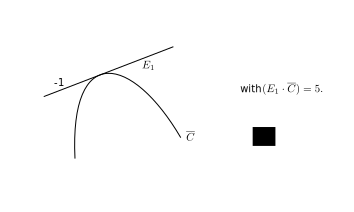
\includegraphics{figures/miyansi_fig32.eps}
\end{figure}
Then we have: $D_{P}=5E_{1}$, $D^{(1)}_{P}=E_{1}$,
$D^{(2)}_{P}=2E_{1}$, $D^{(3)}_{P}=E_{1}$ and $\mu_{P}=\nu_{P}=-1$.

\medskip
\noindent
{\bf Case} $e=7$. $P$ has multiplicity $(5,2,2,1,\ldots)$ and
$\overline{\sigma}^{-1}(P)$ has the configuration:
\begin{figure}[H]
\centering
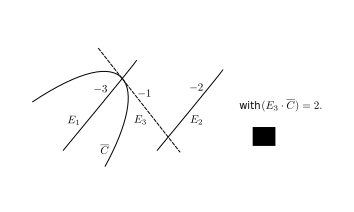
\includegraphics{figures/miyansi_fig33.eps}
\end{figure}
Then\pageoriginale\ we have: $D_{P}=5E_{1}+7E_{2}+14E_{3}$,
$D^{(1)}_{P}=E_{1}+E_{2}$, $D^{(2)}_{P}=2E_{1}+3E_{2}+7E_{3}$,
$D^{(3)}_{P}=E_{1}+2E_{2}+4E_{3}$ and $\mu_{P}=\nu_{P}=-2$.

\medskip
\noindent
{\bf Case} $e=8$. $P$ has multiplicity $(5,3,2,1,\ldots)$ and
$\overline{\sigma}^{-1}(P)$ has the configuration:
\begin{figure}[H]
\centering
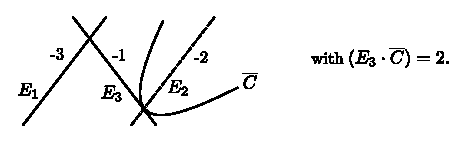
\includegraphics{figures/miyansi_fig34.eps}
\end{figure}
Then we have: $D_{P}=5E_{1}+8E_{2}+15E_{3}$,
$D^{(1)}_{P}=E_{1}+E_{3}$, $D^{(2)}_{P}=2E_{1}+4E_{2}+7E_{3}$,
$D^{(3)}_{P}=E_{1}+2E_{2}+4E_{3}$ and $\mu_{P}=\nu_{P}=-2$.

\medskip
\noindent
{\bf Case} $e=9$. $P$ has multiplicity $(5,4,1,\ldots)$ and
$\overline{\sigma}^{-1}(P)$ has the configuration:
\begin{figure}[H]
\centering
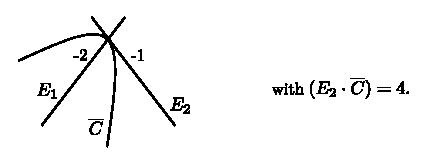
\includegraphics{figures/miyansi_fig35.eps}
\end{figure}
Then we have: $D_{P}=5E_{1}+9E_{2}$, $D^{(1)}_{P}=E_{1}+E_{2}$,
$D^{(2)}_{P}=2E_{1}+4E_{2}$, $D^{(3)}_{P}=E_{1}+2E_{2}$, $\mu_{P}=-1$
and $\nu_{P}=-2$.

We denote by $D$, $D^{(1)}$, $D^{(2)}$, $D^{(3)}$, $\mu$ and $\nu$ the
sum ${\displaystyle{\mathop{\sum}_{P}}}D_{P}$,
${\displaystyle{\mathop{\sum}_{P}}}D^{(1)}_{P}$,
${\displaystyle{\mathop{\sum}_{P}}}D^{(2)}_{P}$,
${\displaystyle{\mathop{\sum}_{P}}}D^{(3)}_{P}$,
${\displaystyle{\mathop{\sum}_{P}}}\mu_{P}$ and
${\displaystyle{\mathop{\sum}_{P}}}\nu_{P}$, respectively, where $P$
runs through all singular points of $C$ lying on $\mathbb{A}^{2}_{k}$.

\subsection{}\label{chap3:3.5}
Now we shall turn to the singular points of $C$ outside of
$\mathbb{A}^{2}_{k}$. It\pageoriginale\ is easy to see that $C$ has
only one point $Q$ outside of $\mathbb{A}^{2}_{k}$ and $C$ is given
locally at $Q$ by
$$
\eta^{d}+\xi^{5}\psi(\eta)=0;\quad Q=(\xi=0,\eta=0)
$$
where $x=1/\xi$, $y=1/\eta$ and $\psi(\eta)=\eta^{d}\varphi(1/\eta)$
with $\psi(0)\neq 0$. We introduce the following notations: Consider a
fibration $\mathscr{F}=\{\ell_{\alpha}:\ell_{\alpha}$ is defined by
$y=\alpha\}$ on $F_{0}$. We denote by $\ell_{\infty}$ the fiber
$y=\infty$ and by $S_{\infty}$ the cross-section $x=\infty$. In the
following we shall compute concretely $(\overline{\sigma}^{\ast}A)$,
$\overline{B}$, $\overline{Z}$, $K_{\overline{F}}$,
$K_{\overline{F}}+\overline{Z}$, $p_{a}(\overline{Z})$ and
$((K_{\overline{F}}+\overline{Z})^{2})$. 

\subsubsection{}\label{chap3:3.5.1}
{\bf Case}~ $d=5n+1$. Then $Q$ is a singular point of multiplicity
$(\underbrace{5,\ldots,5}_{n},1$, $\ldots)$ and
$\overline{\sigma}^{-1}(\ell_{\infty}\cup S_{\infty}\cup C)$ has the
configuration below in a neighborhood of $\overline{\sigma}^{-1}(Q)$:
\begin{figure}[H]
\centering
\includegraphics[scale=1.1]{figures/miyansi_fig36.eps}
\end{figure}
\noindent
with $(E_{n}\cdot\overline{C})=5$ if $n=2m$;
\begin{figure}[H]
\centering
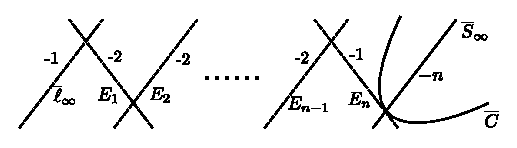
\includegraphics[scale=1.1]{figures/miyansi_fig37.eps}
\end{figure}
\noindent
with $(E_{n}\cdot\overline{C})=5$ if $n=2m+1$, where
$\overline{\ell}_{\infty}:=\overline{\sigma}'(\ell_{\infty})$ and
$\overline{S}_{\infty}:=\overline{\sigma}'(S_{\infty})$. 

We\pageoriginale\ have:
\begin{align*}
  (\overline{\sigma}^{\ast}A) &=\overline{C}+5(E_{1}+2E_{2}+ \cdots +
  nE_{n})+D\\
  & \quad -5(\overline{S}_{\infty} + E_{1}+2E_{2}+\cdots+nE_{n})
   -d(\overline{\ell}_{\infty}+E_{1}+\cdots+E_{n})\\
  &= \overline{C}-5\overline{S}_{\infty}-d~\overline{\sigma}^{\ast}
  (\ell_{\infty})+ \Gamma 
\end{align*}
and
\begin{align*}
E_{\overline{F}} &\sim
-2(\overline{S}_{\infty}+E_{1}+2E_{2}+\cdots+nE_{n})-2(\overline{\ell}_{\infty}+E_{1}+\cdots+E_{n})\\
&\quad +(E_{1}+2E_{2}+\cdots+nE_{n})+D^{(3)}\\
&= -\overline{S}_{\infty}-\overline{\sigma}^{\ast}(S_{\infty})-2\overline{\sigma}^{\ast}(\ell_{\infty})+D^{(3)}.
\end{align*}
Hence we have:

\paragraph{}\label{chap3:3.5.1.1}
{\bf Case} $d=10m+1$ $(n=2m)$.
\begin{align*}
\overline{B} &=
\overline{C}+\overline{S}_{\infty}+\overline{\ell}_{\infty}+E_{1}+\cdots+E_{n}+D^{(1)}\\
\overline{Z} &=
3\overline{S}_{\infty}+(5m+1)\overline{\sigma}^{\ast}(\ell_{\infty})-D^{(2)}\\ 
K_{\overline{F}}+\overline{Z} &\sim
2\overline{S}_{\infty}+(5m-1)\overline{\sigma}^{\ast}(\ell_{\infty})-\overline{\sigma}^{\ast}(S_{\infty})+(D^{(3)}-D^{(2)})\\
&=
\overline{S}_{\infty}+(3m-1)\overline{\sigma}^{\ast}(\ell_{\infty})\\
&\quad +\{2m\overline{\ell}_{\infty}+(2m-1)E_{1}+\cdots+E_{2m-1}\}+(D^{(3)}-D^{(2)})\\
p_{a}(\overline{Z}) &= \frac{1}{2}(\overline{Z}\cdot
K_{\overline{F}}+\overline{Z})+1=4m+\mu\\
((K_{\overline{F}}+\overline{Z})^{2}) &= 2m-2+\nu. 
\end{align*}

\paragraph{}\label{chap3:3.5.1.2}
{\bf Case} $d=10m+6$ $(n=2m+1)$.
\begin{align*}
\overline{B} &= \overline{C}+\overline{S}_{\infty}+D^{(1)}\\
\overline{Z} &=
3\overline{S}_{\infty}+(5m+3)\overline{\sigma}^{\ast}(\ell_{\infty})-D^{(2)}\\
K_{\overline{F}}+\overline{Z} &\sim
2\overline{S}_{\infty}+(5m+1)\overline{\sigma}^{\ast}(\ell_{\infty})-\overline{\alpha}^{\ast}(S_{\infty})+(D^{(3)}-D^{(2)})\\
&=
\overline{S}_{\infty}+3m\overline{\sigma}^{\ast}(\ell_{\infty})+\{(2m+1)\overline{\ell}_{\infty}+2mE_{1}+\cdots+E_{2m}\}\\
&\quad +(D^{(3)}-D^{(2)})\\
p_{a}(\overline{Z}) &= 4m+1+\mu\\
((K_{\overline{F}}+\overline{Z})^{2}) &= 2m-2+\nu.
\end{align*}

\subsubsection{}\label{chap3:3.5.2}
{\bf Case} $d=5n+2$.\pageoriginale\ Then $Q$ has multiplicity
$(\underbrace{5,\ldots,5}_{n},2,2,1,\ldots)$ and
$\overline{\sigma}^{-1}(\ell_{\infty}\cup S_{\infty}\cup C)$ has the
following configuration in a neighborhood of
$\overline{\sigma}^{-1}(Q)$:
\begin{figure}[H]
\centering
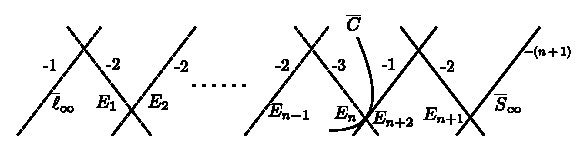
\includegraphics[scale=1.1]{figures/miyansi_fig38.eps}
\end{figure}
\noindent
with $(\overline{C}\cdot E_{n+2})=2$ if $n=2m$;
\begin{figure}[H]
\centering
\includegraphics[scale=1.1]{figures/miyansi_fig39.eps}
\end{figure}
\noindent
with $(\overline{C}\cdot E_{n+2})=2$ if $n=2m+1$. We have:
\begin{align*}
(\overline{\sigma}^{\ast}A) &=
  \overline{C}+5(E_{1}+2E_{2}+\cdots+nE_{n})+(5n+2)E_{n+1}+(10n+4)E_{n+2}+\\ 
  & D-5(\overline{S}_{\infty}+E_{1}+2E_{2} + \cdots+ nE_{n}+ (n+1)
  E_{n+1}+ (2n+1)E_{n+2})\\ 
&\quad
  -d(\overline{\ell}_{\infty}+E_{1}+E_{2}+\cdots+E_{n}+E_{n+1}+2E_{n+2})\\
&=
  \overline{C}-5\overline{S}_{\infty}-d\overline{\sigma}^{\ast}(\ell_{\infty})-3E_{n+1}-E_{n+2}+D 
\end{align*}
and
\begin{align*}
  K_{\overline{F}} &\sim
  -2\overline{\sigma}^{\ast}(S_{\infty})-2\overline{\sigma}^{\ast}
  (\ell_{\infty}) + E_{1}+ 2E_{2}+\cdots+nE_{n}\\
  & \hspace{4cm}+(n+1)E_{n+1} +(2n+2)E_{n+2}+D^{(3)}\\
  &= -\overline{S}_{\infty}-\overline{\sigma}^{\ast} (S_{\infty}) - 2
  \overline{\sigma}^{\ast}(\ell_{\infty})+E_{n+2}+D^{(3)}. 
\end{align*}
Hence\pageoriginale\  we have:

\paragraph{}\label{chap3:3.5.2.1}
{\bf Case} $d=10m+2$ $(n=2m)$.
\begin{align*}
\overline{B} &=
\overline{C}+\overline{S}_{\infty}+E_{n+1}+E_{n+2}+D^{(1)}\\
\overline{Z} &=
3\overline{S}_{\infty}+(5m+1)\overline{\sigma}^{\ast}(\ell_{\infty})+2E_{n+1}+E_{n+2}-D^{(2)}\\
K_{\overline{F}}+\overline{Z} &\sim
2\overline{S}_{\infty}+(5m-1)\overline{\sigma}^{\ast}(\ell_{\infty})-\overline{\sigma}^{\ast}(S_{\infty})\\
& \hspace{2cm}+2E_{n+1}+2E_{n+2}+(D^{(3)}-D^{(2)})\\
&=
\overline{S}_{\infty}+(3m-1) \overline{\sigma}^{\ast} (\ell_{\infty})
+ \{2m\overline{\ell}_{\infty}+(2m-1)E_{1}+\cdots\\
& \qquad +E_{2m-1}+
E_{2m+1}+E_{2m+2}\}+(D^{(3)}-D^{(2)})\\
p_{a}(\overline{Z}) &= 4m+\mu\\
((K_{\overline{F}}+\overline{Z})^{2}) &= 2m-2+\nu.
\end{align*}

\paragraph{}\label{chap3:3.5.2.2}
{\bf Case} $d=10m+7$ $(n=2m+1)$.
\begin{align*}
\overline{B} &=
\overline{C}+\overline{S}_{\infty}+(\overline{\ell}_{\infty}+E_{1}+E_{2}+\cdots+E_{n})+E_{n+2}+D^{(1)}\\
\overline{Z} &=
3\overline{S}_{\infty}+(5m+4)\overline{\sigma}^{\ast}(\ell_{\infty})+E_{n+1}-D^{(2)}\\
K_{\overline{F}}+\overline{Z} &\sim
2\overline{S}_{\infty}+(5m+2) \overline{\sigma}^{\ast} (\ell_{\infty})
-\overline{\sigma}^{\ast}(S_{\infty})+E_{n+1}\\
& \hspace{2cm}+E_{n+2}+(D^{(3)}-D^{(2)})\\
&=\overline{S}_{\infty}+(3m+1) \overline{\sigma}^{\ast}
(\ell_{\infty})\\ 
& \qquad + \{(2m+1)\overline{\ell}_{\infty} + 2mE_{1}+\cdots+E_{2m}\}+(D^{(3)}-D^{(2)})\\
p_{a}(\overline{Z}) &= 4m+2+\mu\\
((K_{\overline{F}}+\overline{Z})^{2}) &= 2m-1+\nu.
\end{align*}

\subsubsection{}\label{chap3:3.5.3}
{\bf Case} $d=5n+3$. Then $Q$ has multiplicity
$(\underbrace{5,\ldots,5}_{n},3,2,1,\ldots)$ and
$\overline{\sigma}^{-1}(\ell_{\infty}\cup S_{\infty}\cup C)$ has the
configuration below in a neighborhood of $\overline{\sigma}^{-1}(Q)$:
\begin{figure}[H]
\centering
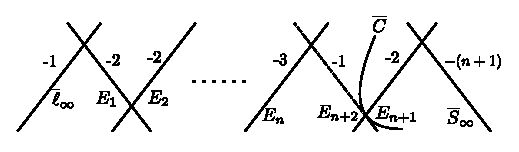
\includegraphics{figures/miyansi_fig40.eps}
\end{figure}
\noindent
with\pageoriginale\ $(\overline{C}\cdot E_{n+2})=2$ if $n=2m$;
\begin{figure}[H]
\centering
\includegraphics{figures/miyansi_fig41.eps}
\end{figure}
\noindent
with $(\overline{C}\cdot E_{n+2})=2$ if $n=2m+1$. We have:
\begin{align*}
(\overline{\sigma}^{\ast}A) &=
  \overline{C}+5(E_{1}+2E_{2}+\cdots+nE_{n}) + (5n+3)E_{n+1}\\ 
  & \hspace{5cm} + (10n+5)E_{n+2}+D\\ 
&\quad  -5(\overline{S}_{\infty}+E_{1} + 2E_{2}+ \cdots + nE_{n}+
  (n+1) E_{n+1}+(2n+1)E_{n+2})\\ 
&\quad
  -d(\overline{\ell}_{\infty}+E_{1}+E_{2}+\cdots+E_{n}+E_{n+1}+2E_{n+2})\\
&= \overline{C}-5\overline{S}_{\infty}-d\overline{\sigma}^{\ast}(\ell_{\infty})-2E_{n+1}+D
\end{align*}
and
\begin{align*}
K_{\overline{F}} &\sim
-2\overline{\sigma}^{\ast}(S_{\infty})-2 \overline{\sigma}^{\ast}
(\ell_{\infty}) + E_{1}+2E_{2}+\cdots+nE_{n}+(n+1)\\
& \hspace{5cm}E_{n+1}+(2n+2)E_{n+2}+D^{(3)}\\
&= -\overline{S}_{\infty}-\overline{\sigma}^{\ast}(S_{\infty})-2\overline{\sigma}^{\ast}(\ell_{\infty})+E_{n+2}+D^{(3)}.
\end{align*}
Hence we have:

\paragraph{}\label{chap3:3.5.3.1}
{\bf Case} $d=10m+3$ $(n=2m)$.
\begin{align*}
\overline{B} &=
\overline{C}+\overline{S}_{\infty}+\overline{\ell}_{\infty}+E_{1}+\cdots+E_{n}+E_{n+1}+D^{(1)}\\
\overline{Z} &=
3\overline{S}_{\infty}+(5m+2)\overline{\sigma}^{\ast}(\ell_{\infty})+E_{n+1}-E_{n+2}-D^{(2)}\\
K_{\overline{F}}+\overline{Z} &\sim
2\overline{S}_{\infty}+5m\overline{\sigma}^{\ast} (\ell_{\infty}) -
\overline{\sigma}^{\ast} (S_{\infty})+E_{n+1}+(D^{(3)}-D^{(2)})\\
&= \overline{S}_{\infty} + (3m-1) \overline{\sigma}^{\ast}
(\ell_{\infty}) + \Big\{(2m+1)\overline{\ell}_{\infty}+2mE_{1} + \cdots +
\\
& \quad  E_{2m}+E_{2m+1}+E_{2m+2}\Big\}+(D^{(3)}-D^{(2)})\\
p_{a}(\overline{Z}) &= 4m+\mu\\
((K_{\overline{F}}+\overline{Z})^{2}) &= 2m-2+\nu.
\end{align*}

\paragraph{}\label{chap3:3.5.3.2}
{\bf Case} $d=10m+8$\pageoriginale\ $(n=2m+1)$.
\begin{align*}
\overline{B} &= \overline{C}+\overline{S}_{\infty}+D^{(1)}\\
\overline{Z} &= 3\overline{S}_{\infty}+(5m+4)\overline{\sigma}^{\ast}(\ell_{\infty})+E_{n+1}-D^{(2)}\\ 
K_{\overline{F}}& +\overline{Z}  \sim  ~2\overline{S}_{\infty} + (5m+2)
\overline{\sigma}^{\ast}(\ell_{\infty})-\overline{\sigma}^{\ast} 
(S_{\infty})+E_{n+1}+E_{n+2}\\
& \hspace{7cm}+ \left(D^{(3)}-D^{(2)}\right)\\
& = \overline{S}_{\infty}+(3m+1)\overline{\sigma}^{\ast}
(\ell_{\infty}) +
\left\{(2m+1)\overline{\ell}_{\infty}+2mE_{1}+\cdots+E_{2m}\right\}\\ 
& \hspace{7cm}+ \left(D^{(3)}-D^{(2)}\right)\\
p_{a}(\overline{Z}) &= 4m+2+\mu\\
((K_{\overline{F}}& +\overline{Z})^{2}) = 2m-1+\nu. 
\end{align*}

\subsubsection{}\label{chap3:3.5.4}
{\bf Case} $d=5n+4$. Then $Q$ has multiplicity
$(\underbrace{5,\ldots,5}_{n},4,1,\ldots)$ and
$\overline{\sigma}^{-1}$ $(\ell_{\infty}\cup S_{\infty}\cup C)$ has the
configuration below in a neighborhood of $\overline{\sigma}^{-1}(Q)$:  
\begin{figure}[H]
\centering
\includegraphics{figures/miyansi_fig42.eps}
\end{figure}
\noindent
with $(\overline{C}\cdot E_{n+1})=4$ if $n=2m$;
\begin{figure}[H]
\centering
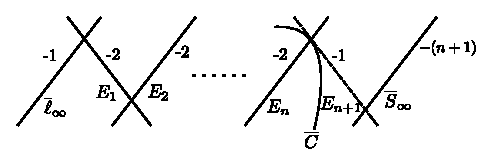
\includegraphics{figures/miyansi_fig43.eps}
\end{figure}
\noindent
with $(\overline{C}\cdot E_{n+1})=4$ if $n=2m+1$. We have:
\begin{align*}
(\overline{\sigma}^{\ast}A) &=
  \overline{C}+5(E_{1}+2E_{2}+\cdots+nE_{n})+(5n+4)F_{n+1}+D\\
&\quad
  -5(\overline{S}_{\infty}+E_{1}+2E_{2}+\cdots+nE_{n}+(n+1)E_{n+1})\\
&\quad -d(\overline{\ell}_{\infty}+E_{1}+E_{2}+\cdots+E_{n}+E_{n+1})\\
&=
  \overline{C}-5\overline{S}_{\infty}-d\overline{\sigma}^{\ast}(\ell_{\infty})-E_{n+1}+D 
\end{align*}\pageoriginale\ 
and
\begin{align*}
K_{\overline{F}} &\sim
-2\overline{\sigma}^{\ast} (S_{\infty})- 2\overline{\sigma}^{\ast}
(\ell_{\infty}) + E_{1}+2E_{2}+\cdots+\\
& \hspace{5cm}nE_{n} +(n+1) F_{n+1}+D^{(3)}\\ 
&= -\overline{S}_{\infty}-\overline{\sigma}^{\ast}(S_{\infty})-2\overline{\sigma}^{\ast}(\ell_{\infty})+D^{(3)}.
\end{align*}
Hence we have:

\paragraph{}\label{chap3:3.5.4.1}
{\bf Case} $d=10m+4$ $(n=2m)$.
\begin{align*}
\overline{B} &= \overline{C}+\overline{S}_{\infty}+E_{n+1}+D^{(1)}\\
\overline{Z} &=
3\overline{S}_{\infty}+(5m+2)\overline{\sigma}^{\ast}(\ell_{\infty})+E_{n+1}-D^{(2)}\\
K_{\overline{F}}+\overline{Z} &\sim
2\overline{S}_{\infty}+5m\overline{\sigma}^{\ast}(\ell_{\infty})-\overline{\sigma}^{\ast}(S_{\infty})+E_{n+1}+(D^{(3)}-D^{(2)})\\
&=\overline{S}_{\infty} + 3m\overline{\sigma}^{\ast} (\ell_{\infty}) +
\{2m\overline{\ell}_{\infty}+(2m-1)E_{1}+\cdots+E_{2m-1}\}\\ 
& \hspace{6.5cm}+(D^{(3)}-D^{(2)})\\
p_{a}(\overline{Z}) &= 4m+1+\mu\\
((K_{\overline{F}}+\overline{Z})^{2}) &= 2m-1+\nu.
\end{align*}

\paragraph{}\label{chap3:3.5.4.2}
{\bf Case} $d=10m+9$ $(n=2m+1)$.
\begin{align*}
\overline{B} &=
\overline{C}+\overline{S}_{\infty}+\overline{\ell}_{\infty}+E_{1}+\cdots+E_{n}+D^{(1)}\\
\overline{Z} &=
3\overline{S}_{\infty}+(5m+5)\overline{\sigma}^{\ast}(\ell_{\infty})-D^{(2)}\\
K_{\overline{F}}+\overline{Z} &\sim
2\overline{S}_{\infty}+(5m+3)\overline{\sigma}^{\ast}(\ell_{\infty})-\overline{\sigma}^{\ast}(S_{\infty})+(D^{(3)}-D^{(2)})\\
&= \overline{S}_{\infty} + (3m+1)\overline{\sigma}^{\ast}
(\ell_{\infty}) + \Big\{(2m+2) \overline{\ell}_{\infty} + (2m+1)\\ 
& \hspace{2cm} E_{1}+ \cdots+ 2E_{2m}+ E_{2m+1}\Big\}+(D^{(3)}-D^{(2)})\\
p_{a}(\overline{Z}) &= 4m+2+\mu\\
((K_{\overline{F}}+\overline{Z})^{2}) &= 2m-2+\nu.
\end{align*}

\subsection{}\label{chap3:3.6}
Next\pageoriginale\ we shall consider the nonsingular minimal model
$\widehat{H}$ of $K$. In the remaining paragraphs of this section we
shall assume for the sake of simplicity that $D^{(2)}=p^{(3)}$. In
view of \ref{chap3:3.4}, this is equivalent to assuming that
$v_{\alpha}(\varphi'(y))\leqq 2$ for every root $\alpha$ of
$\varphi'(y)=0$, and this implies that $\mu=\nu=0$. We shall consider
first {\em the case $m\geqq 1$.} We know in view of \ref{chap3:3.4} and
\ref{chap3:3.5} that $\overline{B}$ has negligible singularities; this
implies that $p_{a}(H)=p_{a}(\overline{Z})>0$ (because $m\geqq 1$) and
$K_{H}\sim \pi^{\ast}(K_{\overline{F}}+\overline{Z})$ (\cf Lemma
\ref{chap3:3.3}); in particular, $H$ is not rational over $k$ and
$\widehat{H}$ exists. In each of the cases enumerated below the
results are obtained by straightforward computations. So, the details
will be omitted.

\subsubsection{}\label{chap3:3.6.1}
{\bf Case} $d=10m+1$. The following assertions hold true:
\begin{enumerate}
\renewcommand{\labelenumi}{(\theenumi)}
\item $(\overline{\sigma}\pi)^{-1}(\ell_{\infty}\cup S_{\infty})$ has
  the next weighted graph:
\begin{figure}[H]
\centering
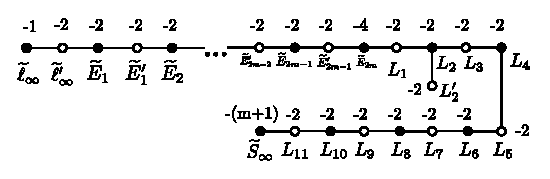
\includegraphics[scale=1.1]{figures/miyansi_fig44.eps}
\end{figure}
\noindent
where
$\pi^{\ast}(\overline{\ell}_{\infty})=2\widetilde{\ell}_{\infty}+\widetilde{\ell}'_{\infty}$,
$\pi^{\ast}(E_{1})=\widetilde{\ell}'_{\infty}+2\widetilde{E}_{1}+\widetilde{E}'_{1}$,
$\pi^{\ast}(E_{i})=\widetilde{E}'_{i-1}+2\widetilde{E}_{i}+\widetilde{E}'_{i}$
for $2\leqq i\leqq 2m-1$,
$\pi^{\ast}(E_{2m})=\widetilde{E}'_{2m-1}+2\widetilde{E}_{2m}+6L_{1}+5L'_{2}+\Sigma^{11}_{i=2}(12-i)L_{i}$
and
$\pi^{\ast}(\overline{S}_{\infty})=2\widetilde{S}_{\infty}+L_{1}+L'_{2}+2
(\Sigma^{11}_{i=2}L_{i})$.

\item
  $\pi^{\ast}(K_{\overline{F}}+\overline{Z})\sim\pi^{\ast}(\overline{S}_{\infty})+(3m-1)\pi^{\ast}\overline{\sigma}^{\ast}(\ell_{\infty})+\{4m\overline{\ell}_{\infty}+(4m-1)\widetilde{\ell}'_{\infty}+(4m-2)\overline{E}_{1}+\cdots+2\widetilde{E}_{2m-1}+\widetilde{E}'_{2m-1}\}$. Since\pageoriginale\
  $K_{H}\sim\pi^{\ast}(K_{\overline{F}}+\overline{Z})$ we know by (1)
  and (2) above that $\widehat{H}$ is obtained from $H$ by contracting
  $\widetilde{\ell}_{\infty}$, $\widetilde{\ell}'_{\infty}$,
  $\widetilde{E}_{1}$,
  $\widetilde{E}'_{1},\ldots,\widetilde{E}_{2m-1}$ and
  $\widetilde{E}'_{2m-1}$. Hence
  $(K^{2}_{\widehat{H}})=2((K_{\overline{F}}+\overline{Z})^{2})+4m=(4m-4)+4m=8m-4$.  
\end{enumerate}

\subsubsection{}\label{chap3:3.6.2}
{\bf Case} $d=10m+2$. The following assertions hold true:
\begin{enumerate}
\renewcommand{\labelenumi}{(\theenumi)}
\item $(\overline{\sigma}\pi)^{-1}(\ell_{\infty}\cup S_{\infty})$ has
  the next weighted graph:
\begin{figure}[H]
\centering
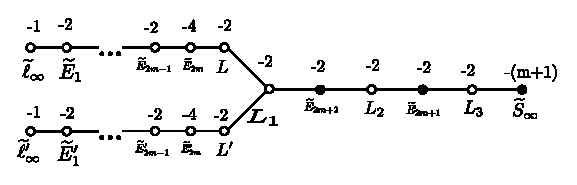
\includegraphics[scale=1.1]{figures/miyansi_fig45.eps}
\end{figure}
\noindent
where
$\pi^{\ast}(\overline{\ell}_{\infty})=\widetilde{\ell}_{\infty}+\widetilde{\ell}'_{\infty}$,
$\pi^{\ast}(E_{i})=\widetilde{E}_{i}+\widetilde{E}'_{i}$ for $1\leqq
i\leqq\leqq 2m-1$,
$\pi^{\ast}(E_{2m})=\widetilde{E}_{2m}+\widetilde{E}'_{2m}+L+L'+L_{1}$,
$\pi^{\ast}(E_{2m+2})=L+L'+2L_{1}+2\widetilde{E}_{2m+2}+L_{2}$,
$\pi^{\ast}(E_{2m+1})=L_{2}+2\widetilde{E}_{2m+1}+L_{3}$ and
$\pi^{\ast}(\widetilde{S}_{\infty})=2\widetilde{S}_{\infty}+L_{3}$. 

\item
  $K_{H}\sim\pi^{\ast}(K_{\overline{F}}+\overline{Z})\sim\pi^{\ast}(\overline{S}_{\infty})+(3m-1)(\overline{\sigma}\pi)^{\ast}(\ell_{\infty})+\{2m\widetilde{\ell}_{\infty}+(2m-1)\widetilde{E}_{1}+\cdots+\widetilde{E}_{2m-1}\}+\{2m\widetilde{\ell}'_{\infty}+(2m-1)\widetilde{E}'_{1}+\cdots+\widetilde{E}'_{2m-1}\}+2\widetilde{E}_{2m+1}+2\widetilde{E}_{2m+2}+L+L'+L_{1}+2L_{2}+L_{3}$. 

Then $\widehat{H}$ is obtained from $H$ by contracting
$\widetilde{\ell}_{\infty}$, 
$\widetilde{E}_{1},\ldots, \widetilde{E}_{2m-1}$ and
$\widetilde{\ell}'_{\infty}$,
$\widetilde{E}'_{1},\ldots,\widetilde{E}'_{2m-1}$. Hence
$(K^{2}_{\widehat{H}})=2((K_{\overline{F}}+\overline{Z})^{2})+4m=(4m-4)+4m=8m-4$. 
\end{enumerate}

\subsubsection{}\label{chap3:3.6.3}
{\bf Case} $d=10m+3$. The following assertions hold true:
\begin{enumerate}
\renewcommand{\labelenumi}{(\theenumi)}
\item $(\overline{\sigma}\pi)^{-1}(\ell_{\infty}\cup S_{\infty})$ has
  the next weighted graph:
\begin{figure}[H]
\centering
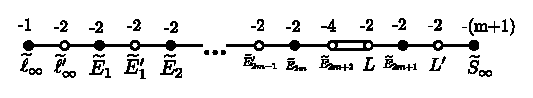
\includegraphics[scale=1.1]{figures/miyansi_fig46.eps}
\end{figure}

\noindent
where\pageoriginale\
$\pi^{\ast} (\overline{\ell}_{\infty})=2\widetilde{\ell}_{\infty}+\widetilde{\ell}'_{\infty}$,
$\pi^{\ast}(E_{1})=\widetilde{\ell}'_{\infty}+2\widetilde{E}_{1}+\widetilde{E}'_{1}$,
$\pi^{\ast}(E_{i})=\widetilde{E}'_{i-1}+2\widetilde{E}_{i}+\widetilde{E}'_{i}$
for $2\leqq i\leqq 2m-1$,
$\pi^{\ast}(E_{2m})=\widetilde{E}'_{2m-1}+2\widetilde{E}_{2m}$,
$\pi^{\ast}(E_{2m+2})=\widetilde{E}_{2m+2}+L$,
$\pi^{\ast}(E_{2m+1})=L+2\widetilde{E}_{2m+1}+L'$ and
$\pi^{\ast}(\overline{S}_{\infty})=L'+2\widetilde{S}_{\infty}$.

\item $K_{H}\sim \pi^{\ast}(K_{\overline{F}}+\overline{Z})\sim
  \pi^{\ast}(\overline{S}_{\infty})+(3m-1)(\overline{\sigma}\pi)^{\ast}(\ell_{\infty})+\{(4m+2)\widetilde{\ell}_{\infty}+(4m+1)\widetilde{\ell}'_{\infty}+4m\widetilde{E}_{1}+(4m-1)\widetilde{E}'_{1}+\cdots+3\widetilde{E}'_{2m-1}+2\widetilde{E}_{2m}\}+\widetilde{E}_{2m+2}+2L+2\widetilde{E}_{2m+1}+L'$. 
\end{enumerate}

Then $\widehat{H}$ is obtained from $H$ by contracting
$\widetilde{\ell}_{\infty}$, $\widetilde{\ell}'_{\infty}$,
$\widetilde{E}_{1},\ldots,\widetilde{E}_{2m}$. Hence
$(K^{2}_{\widehat{H}})=2((K_{\overline{F}}+\overline{Z})^{2})+(4m+1)=(4m-4)+(4m+1)=8m-3$.  

\subsubsection{}\label{chap3:3.6.4}
{\bf Case} $d=10m+4$. The following assertions hold true:
\begin{enumerate}
\renewcommand{\labelenumi}{(\theenumi)}
\item $(\overline{\sigma}\pi)^{-1}(\ell_{\infty}\cup S_{\infty})$ has
  the next weighted graph:
\begin{figure}[H]
\centering
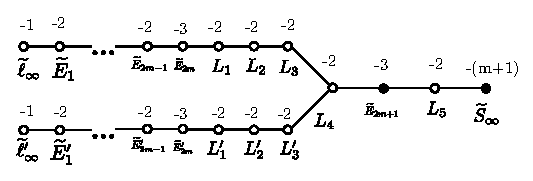
\includegraphics[scale=1.1]{figures/miyansi_fig47.eps}
\end{figure}

\noindent 
where
$\pi^{\ast}(\overline{\ell}_{\infty})=\widetilde{\ell}_{\infty}+\widetilde{\ell}'_{\infty}$,
$\pi^{\ast}(E_{i})=\widetilde{E}_{i}+\widetilde{E}'_{i}$ for $1\leqq
i\leqq 2m-1$,
$\pi^{\ast}(E_{2m})=\widetilde{E}_{2m}+\widetilde{E}'_{2m}+(\Sigma^{3}_{i=1}(L_{i}+L'_{i}))+L_{4}$,
$\pi^{\ast}(E_{2m+1})=(\Sigma^{3}_{i=1}i(L_{i}+L'_{i}))+4L_{4}+2\widetilde{E}_{2m+1}+L_{5}$
and
$\pi^{\ast}(\bar{S}_{\infty})=L_{5}+2\widetilde{S}_{\infty}$.

\item
  $K_{H}\sim\pi^{\ast}(K_{\overline{F}}+\overline{Z})\sim\pi^{\ast}(\overline{S}_{\infty})+3m(\overline{\sigma}\pi)^{\ast}(\ell_{\infty})+\{2m\widetilde{\ell}_{\infty}+(2m-1)\widetilde{E}_{1}+\cdots+\widetilde{E}_{2m-1}\}+\{2m\widetilde{\ell}'_{\infty}+(2m-1)\widetilde{E}'_{1}+\cdots+\widetilde{E}'_{2m-1}\}$. 
\end{enumerate}

Then $\widehat{H}$ is obtained from $H$ by contracting
$\widetilde{\ell}_{\infty}$,
$\widetilde{E}_{1},\ldots,\widetilde{E}_{2m-1}$ and
$\widetilde{\ell}'_{\infty}$,
$\widetilde{E}'_{1},\ldots,\widetilde{E}'_{2m-1}$. Hence
$(K^{2}_{\widehat{H}})=2((K_{\overline{F}}+\overline{Z})^{2})+4m=(4m-2)+4m=8m-2$. 

\subsubsection{}\label{chap3:3.6.5}
{\bf Case} $d=10m+6$. The following assertions hold true:
\begin{enumerate}
\renewcommand{\labelenumi}{(\theenumi)}
\item $(\overline{\sigma}\pi)^{-1}(\ell_{\infty}\cup
  S_{\infty})$\pageoriginale\ has the next weighted graph:
\begin{figure}[H]
\centering
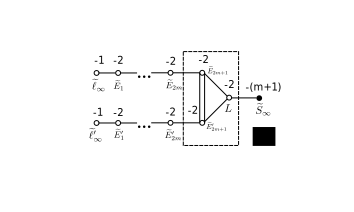
\includegraphics[scale=1.3]{figures/miyansi_fig48.eps}
\end{figure}
\noindent
there components meet in one point with $(\tilde{E}_{2m+1} \cdot
\tilde{E}'_{2m+1})=2$ and $(\tilde{E}_{2m+1} \cdot L) =
(\tilde{E}'_{2m+1}\cdot L)=1$

\noindent
where
$\pi^{\ast}(\overline{\ell}_{\infty})=\widetilde{\ell}_{\infty}+\widetilde{\ell}'_{\infty}$,
$\pi^{\ast}(E_{i})=\widetilde{E}_{i}+\widetilde{E}'_{i}$ for $1\leqq
i\leqq 2m$,
$\pi^{\ast}(E_{2m+1})=\widetilde{E}_{2m+1}+\widetilde{E}'_{2m+1}+L$
and $\pi^{\ast}(\overline{S}_{\infty})=2\widetilde{S}_{\infty}+L$. 

\item $K_{H}\sim \pi^{\ast}(K_{\overline{F}}+\overline{Z})\sim
  \pi^{\ast}(\overline{S}_{\infty})+3m(\overline{\sigma}\pi)^{\ast}(\ell_{\infty})+\{(2m+1)\widetilde{\ell}_{\infty}+2m\widetilde{E}_{1}+\cdots+\widetilde{E}_{2m}\}+\{(2m+1)\widetilde{\ell}'_{\infty}+2m\widetilde{E}'_{1}+\cdots+\widetilde{E}'_{2m}\}$. 
\end{enumerate}

Then $\widehat{H}$ is obtained from $H$ by contracting
$\widetilde{\ell}_{\infty}$,
$\widetilde{E}_{1},\ldots,\widetilde{E}_{2m}$ and
$\widetilde{\ell}'_{\infty}$,
$\widetilde{E}'_{1},\ldots,\widetilde{E}'_{2m}$. Hence
$(K^{2}_{\widehat{H}})=2((K_{\overline{F}}+\overline{Z})^{2})+(4m+2)=(4m-4)+(4m+2)=8m-2$. 

\subsubsection{}\label{chap3:3.6.6}
{\bf Case} $d=10m+7$. The following assertions hold true:
\begin{enumerate}
\renewcommand{\labelenumi}{(\theenumi)}
\item $(\overline{\sigma}\pi)^{-1}(\ell_{\infty}\cup S_{\infty})$ has
  the next weighted graph:
\begin{figure}[H]
\centering
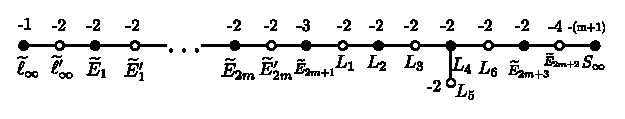
\includegraphics{figures/miyansi_fig49.eps}
\end{figure}
\noindent
where
$\pi^{\ast}(\overline{\ell}_{\infty})=2\widetilde{\ell}_{\infty}+\widetilde{\ell}'_{\infty}$,
$\pi^{\ast}(E_{1})=\widetilde{\ell}'_{\infty}+2\widetilde{E}_{1}+\widetilde{E}'_{1}$,
$\pi^{\ast}(E_{i})=\widetilde{E}'_{i-1}+2\widetilde{E}_{i}+\widetilde{E}'_{i}$
for $2\leqq i\leqq 2m$,
$\pi^{\ast}(E_{2m+1})=\widetilde{E}'_{2m}+2\widetilde{E}_{2m+1}+2(L_{1}+L_{2}+L_{3}+L_{4})+L_{5}+L_{6}$,
$\pi^{\ast}(E_{2m+3})=2\widetilde{E}_{2m+3}+L_{1}+2L_{2}+3L_{3}+4L_{4}+2L_{5}+3L_{6}$,\pageoriginale\
$\pi^{\ast}(E_{2m+2})=\widetilde{E}_{2m+2}$ and
$\pi^{\ast}(\overline{S}_{\infty})=2\widetilde{S}_{\infty}$.

\item $K_{H}\sim
  \pi^{\ast}(K_{\overline{F}}+\overline{Z})\sim\pi^{\ast}(\overline{S}_{\infty})+(3m+1)(\overline{\sigma}\pi)^{\ast}(\ell_{\infty})+\{(4m+2)\widetilde{\ell}_{\infty}+(4m+1)\widetilde{\ell}'_{\infty}+4m\widetilde{E}_{1}+\cdots+2\widetilde{E}_{2m}+\widetilde{E}'_{2m}\}$.
\end{enumerate}

Then $\widehat{H}$ is obtained from $H$ by contracting
$\widetilde{\ell}_{\infty}$, $\widetilde{\ell}'_{\infty}$,
$\widetilde{E}_{1}$, $\widetilde{E}'_{1},\ldots,\widetilde{E}_{2m}$
and $\widetilde{E}'_{2m}$. Hence
$(K^{2}_{\hat{H}})=2((K_{\overline{F}}+\overline{Z})^{2})+(4m+2)=(4m-2)+(4m+2)=8m$. 

\subsubsection{}\label{chap3:3.6.7}
{\bf Case} $d=10m+8$. The following assertions hold true:
\begin{enumerate}
\renewcommand{\labelenumi}{(\theenumi)}
\item $(\overline{\sigma}\pi)^{-1}(\ell_{\infty}\cup S_{\infty})$ has
  the next weighted graph:
\begin{figure}[H]
\centering
\includegraphics[scale=1.3]{figures/miyansi_fig50.eps}
\end{figure}
\noindent
three components meet each other transversely in one point where
$\pi^{\ast}(\overline{\ell}_{\infty})=\widetilde{\ell}_{\infty}+\widetilde{\ell}'_{\infty}$,
$\pi^{\ast}(E_{i})=\widetilde{E}_{i}+\widetilde{E}'_{i}$ for $1\leqq
i\leqq 2m+1$ or $i=2m+3$, $\pi^{\ast}(E_{2m+2})=\widetilde{E}_{2m+2}$
and $\pi^{\ast}(\widetilde{S}_{\infty})=2\widetilde{S}_{\infty}$. 

\item $K_{H}\sim
  \pi^{\ast}(K_{\overline{F}}+\overline{Z})\sim\pi^{\ast}(\overline{S}_{\infty})+(3m+1)(\overline{\sigma}\pi)^{\ast}(\ell_{\infty})+\{(2m+1)\widetilde{\ell}_{\infty}+2m\widetilde{E}_{1}+\cdots+\widetilde{E}_{2m}\}+\{(2m+1)\widetilde{\ell}'_{\infty}+2m\widetilde{E}'_{i}+\cdots+\widetilde{E}'_{2m}\}$. 
\end{enumerate}

Then $\widehat{H}$ is obtained from $H$ by contracting
$\widetilde{\ell}_{\infty}$,
$\widetilde{E}_{1},\ldots,\widetilde{E}_{2m}$ and
$\widetilde{\ell}'_{\infty}$,
$\widetilde{E}'_{1},\ldots,\widetilde{E}'_{2m}$. Hence
$(K^{2}_{\widehat{H}})=2((K_{\overline{F}}+\overline{Z})^{2})+(4m+2)=(4m-2)+(4m+2)=8m$. 

\subsubsection{}\label{chap3:3.6.8}
{\bf Case} $d=10m+9$. The following assertions hold true: 
\begin{enumerate}
\renewcommand{\labelenumi}{(\theenumi)}
\item $(\overline{\sigma}\pi)^{-1}(\ell_{\infty}\cup
  S_{\infty})$\pageoriginale\ has the next weighted graph:
\begin{figure}[H]
\centering
\includegraphics{figures/miyansi_fig51.eps}
\end{figure}
\noindent
where $\Delta$ stands for an irreducible rational curve
$\widetilde{E}_{2m+2}$ with an ordinary cusp $P$ of multiplicity $2$,
$L$ intersects $\widetilde{E}_{2m+2}$ at the cusp point with
$(L\cdot\widetilde{E}_{2m+2})=2$ and $\widetilde{S}_{\infty}$
intersects $\widetilde{E}_{2m+2}$ transversely at a simple point; and
where
$\pi^{\ast}(\overline{\ell}_{\infty})=2\widetilde{\ell}_{\infty}+\widetilde{\ell}'_{\infty}$,
$\pi^{\ast}(E_{1})=\widetilde{\ell}'_{\infty}+2\widetilde{E}_{1}+\widetilde{E}'_{1}$,
$\pi^{\ast}(E_{i})=\widetilde{E}'_{i-1}+2\widetilde{E}_{i}+\widetilde{E}'_{i}$
for $2\leqq i\leqq 2m$,
$\pi^{\ast}(E_{2m+1})=\widetilde{E}'_{2m}+2\widetilde{E}_{2m+1}+L$,
$\pi^{\ast}(E_{2m+2})=L+2\widetilde{E}_{2m+2}$ and
$\pi^{\ast}(\overline{S}_{\infty})=2\widetilde{S}_{\infty}$.

\item $K_{H}\sim
  \pi^{\ast}(K_{\overline{F}}+\overline{Z})\sim\pi^{\ast}(\overline{S}_{\infty})+(3m+1)(\overline{\sigma}\pi)^{\ast}(\ell_{\infty})+\{(4m+4)\widetilde{\ell}_{\infty}+(4m+3)\widetilde{\ell}'_{\infty}+(4m+2)\widetilde{E}_{1}+\cdots+4\widetilde{E}_{2m}+3\widetilde{E}'_{2m}+2\widetilde{E}_{2m+1}+L\}$.  
\end{enumerate}

Then $\widehat{H}$ is obtained from $H$ by contracting
$\widetilde{\ell}_{\infty}$, $\widetilde{\ell}'_{\infty}$,
$\widetilde{E}_{1}$,
$\widetilde{E}'_{1},\ldots,\widetilde{E}_{2m}$, $\widetilde{E}'_{2m},\widetilde{E}_{2m+1}$
and $L$. Hence
$(K^{2}_{\widehat{H}})=2((K_{\overline{F}}+\overline{Z})^{2})+(4m+4)=(4m-4)+(4m+4)=8m$. 

\subsection{}\label{chap3:3.7}
Next we shall consider {\em the case} $m=0$ and assume that
$D^{(2)}=D^{(3)}$. In principle we follow the arguments and
computations done in \ref{chap3:3.5} and \ref{chap3:3.6}. More precisely, the
configurations of $\overline{\sigma}^{-1}(\ell_{\infty}\cup
S_{\infty}\cup C)$ in a neighborhood of $\overline{\sigma}^{-1}(Q)$
are those in \ref{chap3:3.5} up to the following modifications: If
$d=1,2,3,4$ then omit $\overline{\ell}_{\infty}$,
$E_{1},\ldots,E_{n-1}$, put $n=0$ and set anew
$\overline{\ell}_{\infty}:=E_{0}$ and
$(\overline{\ell}^{2}_{\infty})=(E^{2}_{n})+1$; if $d=6,7,8,9$ then
omit $\overline{\ell}_{\infty}$, $E_{1},\ldots,E_{n-1}$, put $n=1$ and
set anew $\overline{\ell}_{\infty}:=E_{0}$ and
$(\overline{\ell}^{2}_{\infty})=(E^{2}_{n-1})+1$. The expressions of
$\overline{B}$, $\overline{Z}$, $K_{\overline{F}}+\overline{Z}$,
$p_{a}(\overline{Z})$ and $((K_{\overline{F}}+\overline{Z})^{2})$ are
obtained from those in \ref{chap3:3.6} by due modifications. 

\subsubsection{}\label{chap3:3.7.1}
{\bf Case} $d=1$.\pageoriginale\ Then $K$ is apparently rational over $k$.

\subsubsection{}\label{chap3:3.7.2}
{\bf Case} $d=2$ (\cf \ref{chap3:3.5.2.1} and \ref{chap3:3.6.2}). Then
$p_{a}(H)=0$ and
$K_{H}\sim(\overline{\sigma}\pi)^{\ast}$ $(S_{\infty}-\ell_{\infty})$. Hence
the bigenus $p_{2}(H)=0$. Thus $H$ is rational over $k$ by
Castelnuovo's criterion of rationality.

\subsubsection{}\label{chap3:3.7.3}
{\bf Case} $d=3$ (\cf \ref{chap3:3.5.3.1} and \ref{chap3:3.6.3}). Then
$p_{a}(H)=0$ and $K_{H}\sim
2\widetilde{S}_{\infty}+L'-\widetilde{E}_{2}-L$. Let $\rho:H\to Y$ be
the contraction of $\widetilde{S}_{\infty}$ and $L'$. Then $K_{Y}\sim
-\rho(E_{2})-\rho(L)$. Hence $p_{a}(Y)=P_{2}(Y)=0$. Thus $Y$ is
rational over $k$, and so is $H$.

\subsubsection{}\label{chap3:3.7.4}
{\bf Case} $d=4$ (\cf \ref{chap3:3.5.4.1} and \ref{chap3:3.6.4}). Then
$p_{a}(H)=1$ and $K_{H}\sim 2\widetilde{S}_{\infty}+L_{5}$. Let
$\rho:H\to Y$ be the contraction of $\widetilde{S}_{\infty}$ and
$L_{5}$. Then $K_{Y}\sim 0$, which implies that $Y$ is a K3-surface
and $Y\cong H$ (the nonsingular minimal model of $K$ over $k$).

\subsubsection{}\label{chap3:3.7.5}
{\bf Case} $d=6$ (\cf \ref{chap3:3.5.1.2} and \ref{chap3:3.6.5}). Then
$p_{a}(H)=1$ and $K_{H}\sim 2\widetilde{S}_{\infty}+L$. Let $\rho:H\to
Y$ be the contraction of $\widetilde{S}_{\infty}$ and $L$. Then
$K_{Y}\sim 0$, which implies that $Y$ is a K3-surface.

\subsubsection{}\label{chap3:3.7.6}
{\bf Case} $d=7$ (\cf \ref{chap3:3.5.2.2} and \ref{chap3:3.6.6}). Then
$p_{a}(H)=2$ and $K_{H}\sim
\pi^{\ast}(\overline{S}_{\infty}+\overline{\ell}_{\infty})+(\overline{\sigma}\pi)^{\ast}(\ell_{\infty})=2\widetilde{\ell}_{\infty}+\widetilde{\ell}'_{\infty}+2\widetilde{S}_{\infty}+(\overline{\sigma}\pi)^{\ast}(\ell_{\infty})$. Let
$\rho:H\to Y$ be the contraction of $\widetilde{S}_{\infty}$,
$\widetilde{\ell}_{\infty}$ and $\widetilde{\ell}'_{\infty}$. Then $Y$
is a minimal surface with $K_{Y}\sim
\rho_{\ast}((\overline{\sigma}\pi)^{\ast}(\ell_{\infty}))$. Hence
$(K^{2}_{Y})=1$. Then $Y$ is a surface of general type.

\subsubsection{}\label{chap3:3.7.7}
{\bf Case} $d=8$ (\cf \ref{chap3:3.5.3.2} and \ref{chap3:3.6.7}). Then
$p_{a}(H)=2$ and $K_{H}\sim
2\widetilde{S}_{\infty}+\widetilde{\ell}_{\infty}+\widetilde{\ell}'_{\infty}+(\overline{\sigma}\pi)^{\ast}(\ell_{\infty})$. Let
$\rho:H\to Y$ be the contraction of $\widetilde{S}_{\infty}$,
$\widetilde{\ell}_{\infty}$ and $\widetilde{\ell}'_{\infty}$. Then $Y$
is a minimal surface with $K_{Y}\sim
\rho_{\ast}((\overline{\sigma}\pi)^{\ast}(\ell_{\infty}))$\pageoriginale\
and $(K^{2}_{Y})=1$. Hence $Y$ is a surface of general type.

\subsubsection{}\label{chap3:3.7.8}
{\bf Case} $d=9$ (\cf \ref{chap3:3.5.4.2} and \ref{chap3:3.6.8}). Then
$p_{a}(H)=2$ and $K_{H}\sim
2\widetilde{S}_{\infty}+4\widetilde{\ell}_{\infty}+3\widetilde{\ell}'_{\infty}+2\widetilde{E}_{1}+L+(\overline{\sigma}\pi)^{\ast}(\ell_{\infty})$. Let
$\rho:H\to Y$ be the contraction of $\widetilde{S}_{\infty}$,
$\widetilde{\ell}_{\infty}$, $\widetilde{\ell}'_{\infty}$,
$\widetilde{E}_{1}$ and $L$. Then $Y$ is a minimal surface with
$K_{Y}\sim \rho_{\ast}((\overline{\sigma}\pi)^{\ast}(\ell_{\infty}))$
and $(K^{2}_{Y})=1$. Hence $Y$ is a surface of general type.

\subsection{}\label{chap3:3.8}
Now it is clear that Theorem \ref{chap3:3.1} is proved in the arguments
of the foregoing paragraphs. In order to show that there exists a
unirational surfaces of general type in characteristic $p>5$ we shall
state the next result without proof.

\begin{prop*}
Let $k$ be an algebraically closed field of characteristic $p>2$. Let
$K:k(t,x,y)$ be the algebraic function field of a hyper surface in
$\mathbb{A}^{3}_{k}$:
$$
t^{2}=x^{p}+y^{p+1}+y^{p-1}+y^{p-2}+\cdots+y^{2}+y.
$$
Then $K$ is rational over $k$ if $p=3$ and irrational over $k$ if
$p\geqq 5$. Let $X$ be the nonsingular minimal model of $K$ over $k$
if $p\geqq 5$. Then $X$ is a unirational $K3$-surface if $p=5$, and
$X$ is a unirational surface of general type with
$p_{a}(X)=(p-1)(p-3)/8$ and $(K^{2}_{X})=(p-5)^{2}/2$ if $p\geqq 7$.
\end{prop*}

\bigskip

\begin{thebibliography}{99}
\bibitem{1} Abhyankar,\pageoriginale\  S.\@ S., Eakin, P., Heinzer, W.: On the uniqueness of
  the ring of coefficients in a polynomial ring. J.\@ Algebra 23
  (1972), 310 - 342.

\bibitem{2} Abhyankar, S.\@ S., Moh, T.\@ T.: Embeddings of the line in the
  plane. J.\@ Reine Angew. Math.\@ 276 (1975), 148 - 166.

\bibitem{3} Abhyankar, S.\@ S., Singh, B.: Embeddings of certain curves in
  the affine plane. Forthcoming.

\bibitem{4} Artin, M.: On Enriques' surfaces: Thesis.\@ (Unpublished).

\bibitem{5} Artin, M.: Some numerical criteria for contractibility of curves
  on algebraic surfaces. Amer.\@ J.\@ math. 84 (1962), 485 - 496.

\bibitem{6} Artin, M.: On isolated rational singularities of
  surfaces. Amer.\@ J.\@ Math. 88 (1966), 129 - 136.

\bibitem{7} Artin, M., Winters, G.: Degenerate fibers and stable reduction
  of curves. Topology 10 (1971), 373 - 383.

\bibitem{8} Ax, J.: Injective endomorphisms of varieties and
  schemes. Pacific J.\@ Math. 31 (1969), 1 - 7.

\bibitem{9} Bombieri, E., Husemoller, D.: Classification and embeddings of
  surfaces. Proc.\@ Sympos.\@ Pure Math. 29 (1975), 329 - 420.

\bibitem{10} Bombieri, E., Mumford, D.: Enriques' classification of surfaces
  in char.\@ p, II. Complex Analysis and Algebraic Geometry. Iwanami
  Shoten Publishers - Cambridge University Press, 1977.

\bibitem{11} Bombieri, E., Mumford, D.: Enriques' classification of surfaces
  in\pageoriginale\ char.\@ p, III. Invent. Math. 36 (1976), 197-232.

\bibitem{12} Chevalley, C.: Introduction to the Theory of Algebraic Functions
  of One Variable.\@ Amer.\@ Math.\@ Soc. Mathematical Surveys 6. New
  York, 1951.

\bibitem{13} Fakin, P., Heinzer, W.: A cancellation problem for
  rings. Lecture Notes in Mathematics. Vol.\@ 311 (pp.\@
  61-77). Berlin-Heidelberg-New York: Springer, 1972.

\bibitem{14} Ganong, R.: On plane curves with one place at
  infinity. Forthcoming.

\bibitem{15} Gieseker, D.: P-ample bundles and their chern classes. Nagoya
  Math.\@ J.\@ 43 (1971), 91-116.

\bibitem{16} Gizatullin, M.H.: On affine surfaces that can be completed by a
  nonsingular rational curve.\@ Izv.\@ Akad.\@ Nauk SSSR, Ser.\@
  Mat.\@ 34 (1970), 778-802; Math.\@ USSR - Izvestija 4 (1970),
  787-810.

\bibitem{17} Grothendieck, A., Dieudonn\'e, J.: El\'ements de G\'eom\'etrie
  Alg\'ebrique.\@ Inst.\@ Hautes Etudes Sci.\@ Publ.\@ Math.\@ 8, 11,
  20, 24, 28, 32.

\bibitem{18} Grothendieck, A.: Fondements de la G\'eom\'etrie Alg\'ebrique -
  extraits du S\'eminaire Bourbaki, 1957-62.\@ Paris: Secr\'etariat
  Math\'ematique. 

\bibitem{19} Grothendieck, A.: S\'eminaire de G\'eom\'etrie Alg\'ebrique (SGA
  2). Amsterdam-paris: North-Holland et Massson, 1968.

\bibitem{20} Grothendieck, A.: Local Cohomology. Lecture Notes in Mathematics
  41. Berlin-Heidelberg-New York: Springer, 1967.

\bibitem{21} Hartshorne, R.: Residues and Duality. Lecture Notes in
  Mathematics 20. Berlin-Heidelberg-New York: Springer, 1966.

\bibitem{22} Hironaka,\pageoriginale\ H.: Smoothing of algebraic cycles of
  small dimensions. Amer.\@ J.\@ Math. 90 (1968), 1-54.

\bibitem{23} Hochster, M.: Non-uniqueness of the ring of coefficients in a
  polynomial ring. Proc.\@ Amer. Math.\@ Soc. 34 (1972), 81-82.

\bibitem{24} Igarashi, T., Miyanishi, M.: Finite subgroups of the
  automorphism group of the affine plane. Forthcoming.

\bibitem{25} Kambayashi, T.: On the absence of nontrivial separable forms of
  the affine plane. J.\@ Algebra 35 (1975), 449-456.

\bibitem{26} Kambayashi, T., Miyanishi, M., Takeuchi, M.: Unipotent Algebraic
  Groups. Lecture Notes in Mathematics 414. Berlin-Heidelberg-New
  York: Springer, 1974.

\bibitem{27} Kambayashi, T., Miyanishi, M.: On Forms of the Affine Line over
  a Field. Lectures in Mathematics, Department of Mathematics, Kyoto
  University, Vol.\@ 20. Tokyo: Kinokuniya Book-Store Co.\@ Ltd.,
  1977.

\bibitem{28} Kambayashi, T., Miyanishi, M.: On flat fibrations by the affine
  line. Illinois J.\@ Math. (to appear).

\bibitem{29} Kodaira, K.: On compact analytic surfaces, II.\@ Ann.\@ of
  Math.\@ 77 (1963), 563-626.

\bibitem{30} Lipman, J.: Rational singularities, with applications to
  algebraic surfaces and unique factorization. Inst.\@ Hautes Etudes
  Sci.\@ Publ.\@ Math. 36 (1969), 195-279.

\bibitem{31} Maruyama, M.: On Classification of Ruled Surfaces. Lectures in
  Mathematics, Department of Mathematics, Kyoto University, Vol.\@
  3. Tokyo: Kinokuniya Book-Store Co.\@ Ltd., 1970.

\bibitem{32} Miyanishi,\pageoriginale\ M.: An algebraic characterization of the affine
  plane. J.\@ Math. Kyoto Univ. 15 (1975), 169-184.

\bibitem{33} Miyanishi, M.: Unirational quasi-elliptic surfaces in
  characteristic 3. Osaka J.\@ Math. 13 (1976), 513-522.

\bibitem{34} Miyanishi, M.: Unirational quasi-elliptic surfaces. Japanese
  J.\@ Math. (New Series) 3. (to appear).

\bibitem{35} Miyanishi, M.: Analytic irreducibility of certain curves on a
  nonsingular affine rational surface. Proc.\@ Internat.\@ Sympos.\@
  on Algebraic Geometry. Kyoto, 1977 (to appear).

\bibitem{36} Miyanishi, M., Nakai, Y.: Some remarks on strongly invariant
  rings. Osaka J.\@ Math. 12 (1975), 1-17.

\bibitem{37} Miyanishi, M., Sugie, T.: Certain affine plane curves with two
  places at infinity. Forthcoming.

\bibitem{38} Moh, T.T.: On analytic irreducibility at $\infty$ of a pencil of
  curves. Proc.\@ Amer.\@ Math.\@ Soc.\@ 44 (1974), 22-24.

\bibitem{39} Mumford, D.: Enriques' classification of surfaces in char.\@ p,
  I.\@ Global Analysis. Princeton University Press, 1969.

\bibitem{40} Nagata, M.: A remark on the unique factorization theorem. J.\@
  Math.\@ Soc.\@ Japan 9 (1957), 143-145.

\bibitem{41} Nagata, M.: Lectures on the Fourteenth Problem of Hilbert. Tata
  Institute of Fundamental Research. Bombay, 1965.

\bibitem{42} Nagata, M.: A theorem on valuation rings and its
  applications. Nagoya Math.\@ J. 29 (1967), 85-91.

\bibitem{43} Nagata, M.: On Automorphism Group of $k[x,y]$. Lectures in
  Mathematics, Department of Mathematics, Kyoto University, Vol.\@
  5. Tokyo: Kinokuniya Book-Store Co.\@ Ltd., 1972.

\bibitem{44} Nakai,\pageoriginale\ Y.: On locally finite iterative higher
  derivations. Osaka J.\@ Math. (to appear).

\bibitem{45} ramanujam, C.P.: A topological characterization of the affine
  plane as an algebraic variety. Ann.\@ of Math. 94 (1971), 69-88.

\bibitem{46} Ramanujam, C.P.: Remarks on the Kodaira vanishing theorem. J.\@
  Indian Math.\@ Soc. 36 (1972), 41-51.

\bibitem{47} Russell, P.: Forms of the affine line and its additive
  group. Pacific J.\@ Math. 32 (1970), 527-539.

\bibitem{48} Russell, P.: Field generators in two variables. J.\@ Math. Kyoto
  Univ. 15 (1975), 555-571.

\bibitem{49} Russell, P.: Simple birational extension of two dimensional
  affine rational domains. Composition Math. 33 (1976), 197-208.

\bibitem{50} Russell, P.: Good and bad field generators. J.\@ Math. Kyoto
  Univ. 17 (1977), 319-331.

\bibitem{51} \v{S}afarevi\v{c}, I.R.\@ et al.: Algebraic Surface. Proc.\@
  Steklov Inst.\@ Math. 75 (1965).

\bibitem{52} Sathaye, A.: On linear planes. Proc.\@ Amer.\@ Math.\@ Soc. 56
  (1976), 1-7.

\bibitem{53} Serre, J.-P.: Groupes finis d'automorphismes d'anneaux locaux
  r\'eguliers. Colloque d'Alg\`ebre.\@ Exp.\@ 8. Paris: Secr\'etariat
  Math\'ematique. 

\bibitem{54} Sweedler, M.E.: A unit theorem applied to Hopf algebras and
  Amitsur cohomology. Amer.\@ J.\@ Math. 92 (1970), 259-271.

\bibitem{55} Tate, J.: Genus change in inseparable extensions of function
  fields. Proc.\@ Amer.\@ Math.\@ Soc. 3 (1952), 400-406.

\bibitem{56} Wright, D.: Cancellation of variables of the form
  $bT^{n}-a$. Preprint.
\end{thebibliography}
